\documentclass{article}

\usepackage{titlesec}
\setcounter{secnumdepth}{4}
\titleformat{\paragraph}
{\normalfont\normalsize\bfseries}{\theparagraph}{1em}{}
\titlespacing*{\paragraph}
{0pt}{3.25ex plus 1ex minus .2ex}{1.5ex plus .2ex}
\usepackage{graphicx}
\graphicspath{ {images/} }
\usepackage{hyperref}
\usepackage{float}
\usepackage{listings}
\begin{document}
\title{Metrics of successful websites and companies}
\author{Danai Avratoglou}
\date{January 2017}
\maketitle
\newpage
\tableofcontents
\newpage
\section{Introduction}
 
An on-line presence of a company was not an important factor of the overall success that the enterprise would have until a few years ago. Taking although into account the vast spread of the impact that internet has on consumers regarding their brand choices and their products this hypothesis is not valid any more. Companies are obliged by the trends to be active on-line and to maintain a website that depicts the image they want their consumers to perceive. By creating a more consumer orientated image they lead the users to create a positive idea regarding the company and this could potentially lead to bigger sales. The purpose of this paper is to understand the relationship that exists between the website of a company and its success. As success we will consider the amount of revenues of the company. Trying to comprehend this relationship a comparison will take place between the enterprises that were deemed as the more successful ones from Fortune 500  based on their revenues and a number of website metrics in order to see by performing regression models and statistical analysis which metrics do affect the most or are related the most with a company's success.
\newpage
\section{Data gathering}
The first step in order to contact this research is to find which companies we are going to examine. Since the purpose of this paper is to see if the website metrics that will be examined are influencing the success of the company it is a good idea to examine websites of some already successful companies and try to find out what they have in common. Thus as it is mentioned in the introduction we will examine the 500 companies that were ranked as the most successful ones from Fortune 500.
\subsection{Data Source - Fortune 500}\label{ds:f500}
The Fortune 500 is an annual list compiled and published by Fortune magazine that ranks 500 of the largest United States corporations by total revenue for their respective fiscal years. The list includes public companies, along with privately held companies for which revenues are publicly available.\cite{key1, key2}\\ 
For the purposes of this paper we will use this list of companies and we will examine their websites in order to understand if they indeed have something in common or if their success is irrelevant with their on-line presence.\\
The first thing that we will need is a list of the names that are include in the fortune 500. The easiest way to obtain this list is from the following article:
\href{url}{http://www.zyxware.com/articles/4344/list-of-fortune-500-companies-and-their-websites}.\ The way that we will obtain the list will be explained further along in this paper.\\
In the following table one can see the 50 most successful companies that are included in the Fortune 500 during the period this paper is taking place. The rest of the list is available in the Appendix A.\ref{appA}
\begin{table}[H]
\centering
\caption{Fortune 500 - 50 first companies}
\begin{tabular}{lll}
\hline
 \\ 1. Walmart 
&  2. Exxon Mobil 
&  3. Apple 
\\ 4. Berkshire Hathaway 
&  5. McKesson 
&  6. UnitedHealth Group 
\\ 7. CVS Health 
&  8. General Motors 
&  9. Ford Motor 
\\ 10. AT\&T 
&  11. General Electric 
&  12. AmerisourceBergen 
\\ 13. Verizon 
&  14. Chevron 
&  15. Costco 
\\ 16. Fannie Mae 
&  17. Kroger 
&  18. Amazon.com 
\\ 19. Walgreens Boots Alliance 
&  20. HP 
&  21. Cardinal Health 
\\ 22. Express Scripts Holding 
&  23. J.P. Morgan Chase 
&  24. Boeing 
\\ 25. Microsoft 
&  26. Bank of America Corp. 
&  27. Wells Fargo 
\\ 28. Home Depot 
&  29. Citigroup 
&  30. Phillips 66 
\\ 31. IBM 
&  32. Valero Energy 
&  33. Anthem 
\\ 34. Procter \& Gamble 
&  35. State Farm Insurance Cos. 
&  36. Alphabet 
\\ 37. Comcast 
&  38. Target 
&  39. Johnson \& Johnson 
\\ 40. MetLife 
&  41. Archer Daniels Midland 
&  42. Marathon Petroleum 
\\ 43. Freddie Mac 
&  44. PepsiCo 
&  45. United Technologies 
\\ 46. Aetna 
&  47. Lowe's 
&  48. UPS 
\\ 49. AIG 
&  50. Prudential Financial 
&
 \\ \hline

\end{tabular}
\end{table}

\subsection{Metrics}
Now that we have declared the companies that we are going to use we will also need to decide which metrics are we going to examine for each site. Since we cannot have access to metrics such as traffic we will have to examine metrics that are more related to how the site is structure and what exactly does the initial page of each site includes. Initially we can divide the metrics in two major categories:
\begin{itemize}
\item What we see?
\item What lays behind of what we see?
\end{itemize}
In the first category we are referring to metrics that can easily be conceived by the naked eye as well. For example the images that a website is using in its landing page. How many there are and if they are big or small.\\
The second category is not so obvious and it includes informations that usually is visible only to the web developer or the creator of the page. The information here are being given from the html code of a site. For instance we can see the actual type and size of an image, an information not visible with the naked eye.\\
Now that we have a first understanding of the two main categories that the metrics we will use are divided in, we can see in detail the metrics that will be examined in this paper:
\subsubsection{Loading time:}\label{M:Loading time}
One aspect of a website that is crucial is the time it takes for it to load. Nowadays that the internet speed is going higher and higher most people do not have the patient to wait for a page to load. That is why we think that a metrics that should be definitely included in this research in the loading time of the initial page of a site.
\subsubsection{Number of links:}\label{M:Number of links}
When someone is browsing through the internet in many cases they are not completely sure what exactly they are looking for and that is why in a website it would be wise to have some links that can direct the user to find what he wants.These links can either direct the user in another page of the same site, in which case the link will be characterized as an internal link. Or they can lead the user to another site, where in that case the link is characterized as an external link.For the purpose of this paper since it is not so clear which type of links are more important to a user we will examine both the internal and the external links.
\subsubsection{Social media:}\label{M:Social media}
Our era is marked by the social media wave that has changed our lifestyle and our daily habits. So it would be considered an overview if we didn't take under consideration the number of social media that the company chooses to participate in. Even though they can also be considered as external links of the website we will examine them separately in order to see if any particular social medium effects the company's revenues.
\subsubsection{Number, type and sizes of images:}\label{M:N,T,S Imgs}
Since the site is the first thing that a user will see for the company and there is a famous quote that says that \textit{"First impressions counts"} we should also examine how the companies decide to visualize their landing page. In other words to see how many images they include in it and more on that what sizes are those images.\\ It is completely different to see only one huge image in the landing page of a site with not many words or descriptions than to see many small images with different information. The purpose is to examine if these type of diversities between the examined websites are actually related to how they are doing profit wise.\\ Moreover a kind of information a little more complicated for a simple user to understand, but plays a very important role in many cases is the type of the image. For example some websites are using specific type of images or banners that are not compatible with all the browsers, leading the user to see some break points in the website and even stop visiting it. That is why we believe is important to review this metric as well.
\subsubsection{Content:} \label{M:Content}
They say a picture worth a thousand words but that is not enough in our case. After exploring the number, sizes and type of pictures that a website is using we should also explore the number of words it is using to accompany the images and complete the outcome that a user will come across. The metrics we will use will be two. The first one will be the total words that are being used in the landing page and the other one will be the total unique words that are being used. When we are referring to unique words we mean words that are not so commonly use such as "a" or "and" and they give an air of individuality to the text. By using this metric we would try to see if the words that are being used are just as important as the actual content and if the words can make a difference.\\
Furthermore we should also take under consideration how comprehending is the text used in the websites for the users. This information can be obtained by calculating the readability index of the website and also the number of sentences that exists in a page (a metric that comes to complete the previous ones).How the readability index is being calculating will be furthered explained in another section.
\subsubsection{HTML Validation:} \label{M:HTML Validation} Moreover we will have to check the quality of the html code behind the website we are seeing. Are there any mistakes in the code for example any brackets that opened and never closed or any links that do not work. We will examine again two different metrics here the number of errors and the number of warnings. The warning are parts of the code that even though they work at the time there is a good chance to malfunction if any changes or addition are to be made to the html code. 
\subsection{Python}
After having a first look into the variables/ metrics we will use in order to contact this research we should now see how we are going to obtain all this information.\\
Since all of this information can be subtract from the html code of a company's website we should use a programming language in order to download the html pages and then to extract the specific metrics we want to examine from them.\\
For the purposes of this paper the programming language that will be used for downloading the metrics from the websites is Python. More specifically the version of Python that will be used is the 2.7 one.\\
Python is a widely used high-level programming language used for general-purpose programming, created by Guido van Rossum and first released in 1991. An interpreted language, Python has a design philosophy which emphasizes code readability (notably using white space indentation to delimit code blocks rather than curly braces or keywords), and a syntax which allows programmers to express concepts in fewer lines of code than possible in languages such as C++ or Java. \\
The language provides constructs intended to enable writing clear programs on both a small and large scale. Furthermore the way that Python allows a user to programming is common to all users which gives this language a leverage as a program build in Python can be easily understood from another user without any difficulty.\\
The environment that is going to be used is from the Anaconda package which is a free open source distribution of the Python and R programming languages for large-scale data processing, predictive analytics, and scientific computing, that aims to simplify package management and deployment. To be more precise from this package we are going to use the Jupyter Notebook.\cite{key4} \\
\subsection{Scripts}
In order to gather all the needed metrics we had to create a variety of small scripts so as to collect them. In this section we will present in detail the procedure and the actual scripts that were used in order to extract the information that later will help us contact the analysis of the relationship between those metrics and the company's status.
\subsubsection{Companies ranking, names and url}
For starters we need to create a list with the names, the ranking and the URL of the sites that we will later download and extract the necessary info from them. So as it was mentioned in the previous section\ref{ds:f500} the first step that needs to be done is to download and gather those informations into a data frame\footnote{a table in Python environment with rows and columns} so as to be able to use them later on.\\
The most easy way to obtain those informations is by extracting them from an already existing list. This list in our case was available in the following link:\href{url}{http://www.zyxware.com/articles/4344/list-of-fortune-500-companies-and-their-websites}.\\
The way to keep only those three informations as three different variables is by separating from the html code of this page the needed information.\\
The first step is to create 3 empty lists where we will include the informations we are going to extract. The first list will contain the rank of each site, the second one will contain the name of the company and the 3rd one will contain the actual link of the company's site:

\begin{center}
\textit{\textbf{Script 1: Initial lists}}
\end{center}
\begin{lstlisting}[language=Python]
list_company_number =[]
list_company_name = []
list_company_website = []
\end{lstlisting}

The second step is to upload some libraries that will help us create this function but also the ones that are going to follow.
\begin{center}
\textit{\textbf{Script 2: Python Libraries}}
\end{center}
\begin{lstlisting}[language=Python]
import urllib
import urllib2
import time
import os
from bs4 import BeautifulSoup
import re
import numpy as np
import pandas as pd
import matplotlib.pyplot as plt
\end{lstlisting}
Finally the third step is to create the function that will firstly download the html code of the url at hand, secondly keep only the part of the code that we need to examine and thirdly save this part into the empty lists we created above. This function is called websites and takes as variable to work only the url of the site we need to examine: 
\begin{center}
\textit{\textbf{Script 3: Companies ranking, names and url}}
\end{center}
\begin{lstlisting}[language=Python]
def websites (url): 
    from time import time
    start = time ()
    browser = urllib2.build_opener() 
    browser.addheaders = [('User-agent', 'Mozilla/5.0')]
    response = browser.open(url)
    myHTML = response.read()
    soup = BeautifulSoup(myHTML,"lxml")    
    o = 0
    td_list =[]
    for row2 in soup.html.body.findAll('td'):
        td_list.insert(o, row2)
        o = o + 1
    a = 0
    b = 1
    c = 2
    list_numbering = 0
    for i in range (0,500):        
        num = str(td_list[a])
        company = str(td_list[b])
        site = str(td_list[c])
        c_num = re.findall('>(.+?)</td>',num)  
        c_num = str(c_num[0])
        c_name = re.findall('>(.+?)</td>',company)
        c_name = str(c_name[0])
        c_site = re.findall('">(.+?)</a>',site)
        c_site = str(c_site[0])        
        list_company_number.insert(list_numbering,c_num)
        list_company_name.insert(list_numbering,c_name)
        list_company_website.insert(list_numbering,c_site)
        a = a + 3
        b = b + 3
        c = c + 3
        list_numbering =  list_numbering + 1 
    end = time ()
    duration = round (end - start, 1)
    minutes = round (duration /60, 1)
    print 'The lists are ready in ', duration, ' seconds'
    print 'The lists are ready in ', minutes, ' minutes'
\end{lstlisting}
The steps we followed to create the following function are the following:
\paragraph{Step 1} We create a fake browser that we are going to use in order to open the page and downloaded. The reason we do that is that many sites do not allow us to download their page because they are afraid of stealing important information. Since we are not using any private information we use this method to avoid issues while trying to open the html page at hand.    
\paragraph{Step 2} We open the url and we read it while saving it in the variable "myHTML".
\paragraph{Step 3} With the help of the Beautiful Soup library\footnote{Beautiful Soup is a Python library for pulling data out of HTML and XML files} we read the page as a lxml file and then for each row of this file we are looking for the "td" parts of the code where the informations we want are included.
\paragraph{Step 4} Since we need the names and the urls of all the 500 sites we created a loop from 0 to 500 where for each i we try to isolate the part of the code that contains the information that we want. Moreover even thought it seems that with this loop we calculate 501 numbers since in Python the second bracket is always open we actually count from zero to 499.
\paragraph{Step 5} We use reg expressions\footnote{A regular expression is a special sequence of characters that helps you match or find other strings or sets of strings, using a specialized syntax held in a pattern.} in order to state precisely what part of the already selected code we want to keep.
\paragraph{Step 6} We insert with a specific order the names, the ranking and the url to the corresponding lists and finally we create a text that will appear when the function is completed. Here we have also calculated the time that this function took to be completed and we will appear it as well along with the text.
\subsubsection{URL validation}
Now that we have saved in the three lists the names, the ranking and the URL of the companies that we are going to examine we first have to check whether or not those URL are valid in order to proceed with the download of the html code behind the initial web page of each one of those companies.\\
We first have to install the validators package in python so as to proceed with the validation of the url. In the command prompt window that opens when you open the Jupyter Notebook you have to write: "pip install validators" and then press enter in order for the package to be installed. This specific package currently supports python versions 2.7, 3.3, 3.4, 3.5 and PyPy.\footnote{https://validators.readthedocs.io/en/latest} 
The function that we are going to use from this package is called validators.url. This functions returns True if the url at hand is a valid url or False if it is not.\\
Below one can see that we created a loop that will run as many time as the length of the list that we created in the previous section.\\
During this loop we create a string variable where we use the URL that we have saved in the list, one at each time, and we add the "http://" prefix.\\
Now that we have create the correct way that a url is supposed to be written we will use the function of the validators package and we will create an if function that will check if the answer to a site is different from True and if it is it would add a unit in the variable nv so as to know at the end how many sites did not had valid URL.\\
Finally we ask from the programme to print the final result so as to know how many URL are not valid. The code that was created for this procedure is the following one:
\begin{center}
\textit{\textbf{Script 4: URL Validation}}
\end{center}
\begin{lstlisting}[language=Python]
nv = 0
for num in range(len(list_company_website)):
    line = 'http://' + str(list_company_website[num])
    x = validators.url(line)    
    if x != True:
        nv = nv +1
print "The validation is complete! There were" , nv,
 "not valid pages"
\end{lstlisting}
In our case all the URL where valid so we are eligible to proceed at the next part of the code.
\subsubsection{Download sites html code}
After checking the validity of the URL that we have saved in the list the next step is to download the actual html code of the initial pages of each one of the 500 websites we want to examine.\\
As we did in the section 2.4.1 we have to create a fake browser so as the to be able to download the html code without contacting any problems. In our case we created a Mozilla browser.\\
In order for the url to be opened we must first bring it to the correct form. Initially we create again a loop and for each loop we will examine a specific url. We first replace some symbols on the string that will not be recognized if we try to open the url in this form and then we add the "http://" in the begging of each url.\\ 
Before starting downloading we create some rules for some exceptions. For example the sites 71 (Best Bay),119 (Arrow Electronics) and 465 (St. Jude Medical) in ranking create problem when we tried to download them and the code is stop working. So in order to avoid such incidents we created an exception and the python code will not even try to download these sites and in their position in the new list with the html pages that we will create a zero will be saved.The same thing would happen if an exception is thrown in the function if that we are creating. In any other case we will open the site and save this action in the variable response2.\\
After saving the action we will use the command read and we will save the html code which is essentially a long piece of text and then we will save this "text" in the list.\\
Finally we will wait for 2 seconds in order for the browser not to be suspicious from the extreme speed that we are going to open the next page. In that way we avoid having any crushing incidents on the code.\\
After completing this procedure for all the site we will have a list that in each position the html code will be held as a very large text. Except from the sites that were not able to be opened.\\
The code that was created for this procedure is the following:
\begin{center}
\textit{\textbf{Script 5: Download sites HTML}}
\end{center}
\begin{lstlisting}[language=Python]
import time
browser2 = urllib2.build_opener()
browser2.addheaders = [('User-agent', 'Mozilla/5.0')]
for i in range (0,500):
    k = str(i + 1)
    lc = str(list_company_website[i])
    lc = lc.replace("'","")
    lc = lc.replace("[","")
    lc = lc.replace("]","")
    lcn = str(list_company_name[i])
    lcn = lcn.replace("'","")
    lcn = lcn.replace("[","")
    lcn = lcn.replace("]","")
    url2= 'http://' + lc
    list500_names.insert(i,lcn)
    list500_url.insert(i,lc)
    list500_num.insert(i,k)
    if i == 118 or i == 464 or i == 70:
        list500_sites.insert(i,0)  
        print ("The site " + str(i) 
        + " has NOT been downloaded!")
    else:
        try:
            response2=browser2.open(url2)
            print ("The site " + str(i) 
            + " has been downloaded!")
        except Exception:
            list500_sites.insert(i,0)
            print ("The site " + str(i) 
            + " has NOT been downloaded from exception!")           
            continue 
        myHTML2=response2.read()
        list500_sites.insert(i,myHTML2)        
        time.sleep(2)         
\end{lstlisting}
\subsubsection{Not downloadable pages}
As we explained in the previous section there are some pages that were not able to be downloaded. In order to know which are those pages and more specifically which companies sites will not be available for further exploration we created this part of the code which creates a list with the names of those companies.\\
In the previous code we used a zero in each position that we weren't able to download the site. Here we will use this information in order to gather in a new list only the parts of the list that did get a zero.\\
Here we actually created a small function that is called $"not_downloadables"$. In the first part of the code we create the function and in the second part we run the function for our lists. Finally we create a data frame with the results so as to be more easy on the eyes.\\
The code that was created is the following:
\begin{center}
\textit{\textbf{Script 6: Not downloadable HTML}}
\end{center}
\begin{lstlisting}[language=Python]
not_d = []
not_d_n = []
num = []
def not_downloadables (list500_names,list500_sites):
    met = 0       
    for i in range(len(list500_names)):       
        if list500_sites[i] == 0:
            ct = list500_names[i]
            not_d.insert(met,ct)
            not_d_n.insert(met,str(i))
            num.insert(met,met)
            met = met + 1

not_downloadables (list500_names,list500_sites)

d = {'company' : pd.Series(not_d, index=[num]),
     'number' : pd.Series(not_d_n, index=[num])}
nd = pd.DataFrame(d)    
nd
\end{lstlisting}
In the following table we can see the sites that were not downloaded: 
\begin{table}[H]
\centering
\caption{Not downloadable sites}
\begin{tabular}{ll}
\hline
 &  \\ 
16. Fannie Mae 
& 63. HCA Holdings \\
71. Best Buy
& 91. Nike \\
98. Tesoro 
& 119. Arrow Electronics\\
136. AutoNation
& 142. Southwest Airlines \\
162. Southern 
& 165. American Electric Power\\
196. Office Depot 
& 217. PBF Energy \\
229. Consolidated Edison
& 240. Toys “R” Us \\
243. Dominion Resources 
& 276. Global Partners\\
307. PayPal Holdings 
& 327. News Corp. \\
364. Williams 
& 415. Tractor Supply\\ 
442. Old Republic International 
& 465. St. Jude Medical \\
\hline

\end{tabular}
\end{table}
\subsubsection{Content}\label{content}
Now that we have downloaded the html code we should start extracting some of the variables we are going to use for the analysis in the next chapter.\\
The first thing we are going to check is how easy it is for a user to read the content of each site. In order to check this performance indicator we will need to gather 4 variables:
\begin{enumerate}
\item Number of Words
\item Number of Unique Words
\item Number of Sentences
\item Flesch score
\end{enumerate}
The three first are quite clear. The number of words are the total words that appear in the texts that the user is seeing in a website. The number of unique words are the words that are not very common and can attract the readers attention or even make it harder for him to comprehend the text. The number of sentences is related to those variables as we can understand from this is comparison to the number of total words how big or short is the sentence and as a conclusion how easy or not is the complete text.\\
Finally regarding the forth variable the flesh score is referring to the Flesh reading ease test score.In the Flesch reading-ease test, higher scores indicate material that is easier to read; lower numbers mark passages that are more difficult to read. The formula for the Flesch reading-ease score (FRES) test is:\\ \\
$206.835 - 1.015 (total words/total sentences) - 84.6 (total syllables/total words)$\\
\\
We will calculate the flesh reading test and the other three aforementioned variables with the help of an on-line checking site called: \\
"http://www.webpagefx.com/tools/read-able/".\\
This site calculates and return all these results that we need. The way to implement them in a new data frame to our python code is by dividing the html code, behind the page with the results for each site, and keeping only the actual numbers and sizes that we seek. \\
\begin{center}
\textit{\textbf{Script 7: Content}}
\end{center}
\begin{lstlisting}[language=Python]
flesch = []
sentence = []
word = []
unique_w =[]
empty =[]

import time 
for num in range(0,500):
    site = list500_sites[num]
    line = list500_url[num] 
    url_check = "http://www.webpagefx.com/tools/
    read-able/check.php?tab=Test+By+Url&uri=http://"+ line
    browser = urllib2.build_opener()
    browser.addheaders = [('User-agent', 'Mozilla/5.0')]
    if site == 0 or num == 107:
        print("Site", str(num), "is not validated from sites")
        flesch.insert(num,"n/a")
        sentence.insert(num,"n/a")
        word.insert(num,"n/a")
        unique_w.insert(num,"n/a")  
    else:
        try:
            response = browser.open(url_check)
        except Exception: 
            flesch.insert(num,"n/a")
            sentence.insert(num,"n/a")
            word.insert(num,"n/a")
            unique_w.insert(num,"n/a")
            print("Site", str(num), "is not validated from check")
            continue        
        html_r = response.read()
        check = str(html_r)       
        if check != empty:                
                soup = BeautifulSoup(check,"lxml")
                o = 0
                keyf = []
                for row in soup.html.body.findAll('tr'):
                    keyf.insert(o,row)
                    o = o + 1
                if keyf != empty:                        
                        print("Site", str(num), "is validated")
                        #Flesh measurement
                        if keyf[0] != empty:
                            readability = str(keyf[0])
                            split1 = readability.split('>')
                            readability2 = str(split1[4])
                            split2 = readability2.split('<')
                            readability3 = str(split2[0])
                            flesch.insert(num,readability3)
                        else:
                            flesch.insert(num,"n/a")
                            sentence.insert(num,"n/a")
                            word.insert(num,"n/a")
                            unique_w.insert(num,"n/a")   
                        #Number of sentences   
                        if keyf[6] != empty:
                            sentences = str(keyf[6])
                            spli1 = sentences.split('>')
                            sentences2 = str(spli1[4])
                            spli2 = sentences2.split('<')
                            sentences3 = str(spli2[0])
                            sentence.insert(num,sentences3)
                        else:
                            flesch.insert(num,"n/a")
                            sentence.insert(num,"n/a")
                            word.insert(num,"n/a")
                            unique_w.insert(num,"n/a")  
                        #Number of words
                        if keyf[7] != empty:
                            words = str(keyf[7])
                            spl1 = words.split('>')
                            words2 = str(spl1[4])
                            spl2 = words2.split('<')
                            words3 = str(spl2[0])
                            word.insert(num,words3)
                        else:
                            flesch.insert(num,"n/a")
                            sentence.insert(num,"n/a")
                            word.insert(num,"n/a")
                            unique_w.insert(num,"n/a")  
                        #No. of complex words
                        if keyf[7] != empty:
                            unique_ws = str(keyf[8])
                            sp1 = unique_ws.split('>')
                            unique_ws2 = str(sp1[4])
                            sp2 = unique_ws2.split('<')
                            unique_ws3 = str(sp2[0])
                            unique_w.insert(num,unique_ws3)
                        else:
                            flesch.insert(num,"n/a")
                            sentence.insert(num,"n/a")
                            word.insert(num,"n/a")
                            unique_w.insert(num,"n/a")  
                else:
                        print("Site", str(num), "is not validated from check 2")
                        flesch.insert(num,"n/a")
                        sentence.insert(num,"n/a")
                        word.insert(num,"n/a")
                        unique_w.insert(num,"n/a")            
    time.sleep(2)
\end{lstlisting}
\textbf{Step 1} \\We create four lists where we will save the variables that we are looking for. Then we start a loop for the 500 sites where in each loop we change the value of the 3 main variables the sites that contain the html code the url that contain the url of the company at hand each time and the url check where we save the part of the web address that remains the same while doing the on line check and we add at the end the url of the site we want to check. Also we open the browser as we have done in previous scripts as well.\\\\
\textbf{Step 2} \\Then we create an if part where we check that the variable site is not zero and that we will not examine the site 108 (Tech Data) as the code seems to have a problem in that case. In this check we put on the respective sites n/a values so as to be clear that we did not retrieve these info for them.\\\\
\textbf{Step 3} \\We open the browser link and we check whether or not we drop to any exception in which case we also put n/a values in the respective companies.\\\\
\textbf{Step 4} \\We read the link and after checking that it is not empty (this we  can check by comparing it with an empty list that we have created for this use) we use the Beautiful soup library to extract the part of the code that we need.\\\\
\textbf{Step 5} \\After taking a look at the html code of the pages we find out that the parts that we need are between the following brackets <tr>...</tr> so we will extract each such bracket from the code and save them in a list. By checking the list we found which numbers of the list items we want and we saved them in the variables we have created. Always of course checking first that the specific prices exist or in any other way we again put n/a.\\\\
\textbf{Step 6} \\Now that we have the for key indicators that we will use later on the analysis we should also create a more easily comprehend variable that is related to the flesh measure variable we just created. The numbers that each site gathered mean different things. So we will try to create a correlation and build a variable called readability that will say in text how easily read or not a site is. The score can be interpreted by the following logic:
\begin{itemize}
\item Flesch measure $<$ 30 : Very Confusing
\item Flesch measure $>$ 30 : Difficult
\item Flesch measure $>$ 50 : Fairly Difficult
\item Flesch measure $>$ 60 : Standard
\item Flesch measure $>$ 70 : Fairly Easy
\item Flesch measure $>$ 80 : Easy
\item Flesch measure $>$ 90 : Very Easy
\end{itemize}
\textbf{Step 7} \\
We created a function that creates a new list where the flesh measure variable is being saved as the above descriptions based on the scores each of the site achieved.\\\\
\textbf{Step 8} \\
Now that we have all the needed informations in lists we should combine them by creating one data frame with the use of the variable company name again in order to have a common key so as to merge all the data frames that we will create in the end.
\begin{center}
\textit{\textbf{Script 8: Readability variable}}
\end{center}
\begin{lstlisting}[language=Python]
readability = []
def readable (flesch):
    for i in range (len(flesch)):
            f_n = flesch[i]
            if f_n == "n/a":
                readability.insert(i,"n/a")                
            else:
                a = int(float(f_n))
                if a > 90:    
                    readability.insert(i,"Very easy")                    
                elif a > 80:
                    readability.insert(i,"Easy")
                elif a > 70:
                    readability.insert(i,"Fairly easy")
                elif a > 60:
                    readability.insert(i,"Standard")
                elif a > 50:
                    readability.insert(i,"Fairly difficult")
                elif a > 30:
                    readability.insert(i,"Difficult")
                else:
                    readability.insert(i,"Very Confusing")                    
    print "The function is completed!"

readable (flesch)

d1 = {'company' : pd.Series(list500_names, index=[list500_num]),
      'url' : pd.Series(list500_url, index=[list500_num]),
      'Readability' : pd.Series(readability, index=[list500_num]),
      'Flesh_Mesaure' : pd.Series(flesch,index=[list500_num]),
'Sentences' : pd.Series(sentence, index=[list500_num]),
'Words' : pd.Series(word, index=[list500_num]),
'Unique words' : pd.Series(unique_w, index=[list500_num])}
fre = pd.DataFrame(d1)    
\end{lstlisting}
\subsubsection{HTML Validation}
After downloading and saving in data frames the first batch of metrics that we will need for the analysis that we will do further along we should also check the quality of the html code.\\
Most pages on the World Wide Web are written in computer languages (such as HTML). One of the advantages of writing in a computer language is that it allows the developer to structure text, add multimedia content, and specify what appearance, or style, the result should have based on his needs.\\
As every speaking language,so the computer languages do have their own grammar, vocabulary and syntax too. Each document that is written in these computer languages is supposed to follow these rules in order to consider it well structure and written.\\
However, just as texts in a natural language can include spelling or grammar errors, documents using computer languages may (for various reasons) not be following these rules as well.\\
The process of verifying whether or not a document actually follows the rules for the language it uses is called validation, and the tool used for that is a validator. A document that passes this process with success is called valid.\\
With these concepts in mind, we can define "validation" as the process of checking a web document against the grammar (generally a DTD\footnote{DTT: Document Type definition}) it claims to be using.\\
For the purposes of this paper we will use an on-line validator site called W3C\footnote{https://validator.w3.org/} which will help as see how many errors and warnings does each site have. \\\\
\textbf{Step 1}\\
Initially we create the empty lists in which we will save the variables we will extract that will give as a clear glance on how many errors does each page has, how many warnings, how many pages weren't recognized as documents and how many pages did open during the process.\\\\
\textbf{Step 2}\\
The next step is to create a function that will do a similar job as the script we used to extract the previous variables. Initially we locate the part of the url that remains the same when the check is completed and we see the part that does change where the name of the url we want to examine should go. In order for the code to recognize that we save the result in a variable that in the end is a new url that when we open it, it will show as the page of the results for each site in each loop that we are examining.\\\\
\textbf{Step 3}\\
One difference in this script is that now the part of the code that we need is not between <tr>..</tr> but between <div>...</div> parts of the code. So we follow the same procedure as before and we locate in the list of all the divs that we create with the help of the Beatuful soup package the parts that gives us the informations we want to keep.\\\\
\textbf{Step 4}\\
One other difference is that here after the procedure ends we have counted the actual time we needed to complete this procedure. Then next step is to run the function we created.\\\\
\textbf{Step 5}\\
Finally we save the lists that we created in a new data frame where the common column remains the name of the company as it already is in the previous dataframes we have created.
\begin{center}
\textit{\textbf{Script 9: HTML Validation}}
\end{center}
\begin{lstlisting}[language=Python]
num_errors = []
num_info_warnings = []
num_non_doc = [] 
nm = []
num_open_page = []
empty = ""
 
def html_validation (list500_url,list500_names):
    from time import time # I used it to see how much time it does to run the function
    start = time ()
    for num in range(len(list500_names)):
        line = list500_url[num] 
        url_check = "https://validator.w3.org/nu/?doc=https://" + line
        browser = urllib2.build_opener()
        browser.addheaders = [('User-agent', 'Mozilla/5.0')]
        response = browser.open(url_check)
        html_check = response.read()
        html_check
        check = str(html_check)
        er = 0
        err = 0
        errr = 0
        e = False
        if check != empty:
            e = True
            soup = BeautifulSoup(check,"lxml")
            o = 0
            keyf = []
            for row in soup.html.body.findAll('div'):
                keyf.insert(o,row)
                o = o + 1                    
            if len(keyf) != 0:       
                    keyfin = str(keyf[2])                     
                    dol= re.findall('class="error"',keyfin)            
                    er = er + len(dol)
                    doll= re.findall('class="info warning"'
                                     ,keyfin)            
                    err = err + len(doll)
                    dolll= re.findall('class="non-document-error io"'
                                      ,keyfin)            
                    errr = errr + len(dolll)
        num_errors.insert(num,er)
        num_info_warnings.insert(num,err)
        num_non_doc.insert(num,errr)  
        nm.insert(num,num) 
        num_open_page.insert(num,e)
    end = time ()
    duration = round (end - start, 3)
    minutes = round (duration /60, 1)
    print 'The lists are ready in ', minutes, ' minutes'
 

html_validation (list500_url,list500_names)
 

d8 = {'company' : pd.Series(list500_names, index=[nm]),
      'The_page_opened' : pd.Series(num_open_page, index=[nm])
      ,'number_of_errors' : pd.Series(num_errors, index=[nm]),
      'number_of_warning' : pd.Series(num_info_warnings, index=[nm])
      ,'non-document-error' : pd.Series(num_non_doc, index=[nm])}
html_val = pd.DataFrame(d8)    
html_val.head(3) 
\end{lstlisting}
\subsubsection{Social media}
One other group of variables that we should include in our analysis is the social media that each company choose to use. Since this era is being characterized from the massive use of social media we can't help but wonder if some of them could actually play a crucial role in a business success.\\
The way we are going to see which social media does a company use is quite simple. We will create a list with the name of each of the  six most well known social media with the suffix ".com" and then we will check if the expression appears in the html code of each company. If an expression does exists that means that the specific company does indeed uses this specific social media and as so it appears a respective link in it's home page so as the user to have the opportunity to subscribe in it.\\
The procedure we will use is similar to the previous ones. Firstly we create the lists for the social media that we want to examine. More specifically the social media we will search for are the following:
\begin{itemize}
\item\textbf{Facebook}: a social media that lets you upload images, thoughts, songs and lets you interact with your friends
\item\textbf{Twitter}: an on-line news and social networking service where users post and interact with messages, "tweets," restricted to 140 characters
\item\textbf{Pinterest}: an internet photo sharing and publishing service that allows users to "Pin" pictures they like and upload their own recommendations to their "pinboards".
\item\textbf{YouTube}: a free video sharing website that lets people upload, view, and share videos. 
\item\textbf{Instagram}: an online photo and video sharing social networking service. It allows users to take pictures and videos, apply digital filters to them and share them to their followers. 
\item\textbf{Linkedin}: a social networking website for people in professional jobs. Users can make connections with other people they have worked with, post their work experience and skills, look for jobs, and look for workers.
\end{itemize}
The next step is to create a function that first creates the lists with the 6 elements we would search on each html code. Then after checking that the html code for each specific site has been downloaded properly (in other words is not equal to zero) we search in a loop for each of the social media at hand if it exists in the html code. If it exists we put True in the respective list.After completing this procedure we export also the time we did to run the function.\\
Now that we have the function ready we run it and afterwards we again save the results in a new data frame.
\begin{center}
\textit{\textbf{Script 10: Social media variables}}
\end{center}
\begin{lstlisting}[language=Python]
sm_f = []
sm_t = []
sm_i = []
sm_p = []
sm_y = []
sm_l = []   
sm_nm = [] 
nm = []
sm_url = []
 
def socialmedia (list500_sites,list500_names,list500_url):
    from time import time 
    start = time ()
    for i in range(len(list500_names)):        
            myHTML = list500_sites[i]
            sm = ['facebook.com','twitter.com',
                  'instagram.com','pinterest.com',
                  'youtube.com','linkedin.com'] 
            if myHTML == 0:
                sm_nm.insert(i,list500_names[i]) 
                nm.insert(i,i)
                sm_url.insert(i,list500_url[i])
                sm_f.insert(i,'n/a')
                sm_t.insert(i,'n/a')
                sm_i.insert(i,'n/a')
                sm_p.insert(i,'n/a')
                sm_y.insert(i,'n/a')
                sm_l.insert(i,'n/a')
            else:
                for index in range(len(sm)):
                    x = sm[index]
                    social = re.findall(x,myHTML)                                
                    if (len(social) > 0):
                        if x == 'facebook.com':
                            answerf = 'TRUE'
                        if x == 'twitter.com':
                            answert = 'TRUE'
                        if x == 'instagram.com':
                            answeri = 'TRUE'
                        if x == 'pinterest.com':
                            answerp = 'TRUE'
                        if x == 'youtube.com':
                            answery = 'TRUE'
                        if x =='linkedin.com':
                            answerl = 'TRUE'                   
                    else:
                         if x == 'facebook.com':
                            answerf = 'FALSE'
                         if x == 'twitter.com':
                            answert = 'FALSE'
                         if x == 'instagram.com':
                            answeri = 'FALSE'
                         if x == 'pinterest.com':
                            answerp = 'FALSE'
                         if x == 'youtube.com':
                            answery = 'FALSE'
                         if x =='linkedin.com':
                            answerl = 'FALSE'                
                sm_nm.insert(i,list500_names[i]) 
                nm.insert(i,i)
                sm_url.insert(i,list500_url[i])
                sm_f.insert(i,answerf)
                sm_t.insert(i,answert)
                sm_i.insert(i,answeri)
                sm_p.insert(i,answerp)
                sm_y.insert(i,answery)
                sm_l.insert(i,answerl)
    end = time ()
    duration = round (end - start, 3)
    minutes = round (duration /60, 1)
    print 'The lists are completed in ', minutes, ' minutes' 
    print 'The lists are ready in ', duration, ' seconds'
 
socialmedia (list500_sites,list500_names,list500_url)

d2 = {'company' : pd.Series(sm_nm, index=[nm]),
     'facebook' : pd.Series(sm_f, index=[nm]),
      'twitter' : pd.Series(sm_t, index=[nm]),
     'instagram' : pd.Series(sm_i, index=[nm]),
      'pinterest' : pd.Series(sm_p, index=[nm]),
     'youtube' : pd.Series(sm_y, index=[nm]),
      'linkedin' : pd.Series(sm_l, index=[nm]),}
social_media = pd.DataFrame(d2) 
\end{lstlisting}
\subsubsection{Links - Internal and External}
Next step is to see how many internal, external and finally total links each html code has. The links show in how many other pages does this home page leads to. If the links are external that means as we said before that they lead in a page that is not of this website. While the internal links lead to other pages in the same website.\\
By extracting this information we want to see if it is important for the user to have the ability to browse in various pages inside the site from the home page and also if it plays any role the use of external links that give the user the opportunity to be transferred in another site that is relative of course with the one he is looking in.\\
One easy way to spot the links in an html code is the prefix that they all use which is "href". So the first step (after creating the initial lists of course and the loop we do in each script) is to locate how many times does the expression "href" appears in the code. The result of this search will give us the total links of the site.\\
Next step is to separate somehow the internal and the external ones. An easy way to do that is to find all the "href" references that are followed by "="https: ". By locating specifically those expressions we have located all the external links because unlike the internal links that do not need to be written in this form the external links since they lead to other sites they should always begin with this expression.\\
Now that we have the total links and the external links as well we can easily find the internal links with a simple subtraction.:\
\begin{center}
\textit{total links - external links = internal links}
\end{center}
Finally we put the results in the respective lists for each site and we export the time we did to run the script.\\
Now that the function is completed we run it and then we create a data frame as we have done in the previous scripts as well.
\begin{center}
\textit{\textbf{Script 11: Links Internal and External variables}}
\end{center}
\begin{lstlisting}[language=Python]
l_nm = []
l_ex = []
l_in = []
l_t = []
nm = []
l_url = []


def links (list500_sites,list500_names,list500_url):
    from time import time    
    start = time ()
    for num in range(len(list500_names)):        
            myHTML = list500_sites[num]
            if myHTML == 0:
                l_nm.insert(num,list500_names[num])            
                l_ex.insert(num,'n/a')
                l_t.insert(num,'n/a')
                l_in.insert(num,'n/a')
                nm.insert(num,num)                
            else: 
                href = re.findall('href',myHTML)
                external = re.findall('href="https:',myHTML)
                ex = (len(external))
                alllinks = (len(href))
                internal =  (len(href) - len(external))
                l_nm.insert(num,list500_names[num])            
                l_ex.insert(num,ex)
                l_t.insert(num,alllinks)
                l_in.insert(num,internal)
                nm.insert(num,num)                
    end = time ()
    duration = round (end - start, 3)
    minutes = round (duration /60, 1)
    print 'The lists are ready in ', minutes, ' minutes'
    print 'The lists are ready in ', duration, ' seconds'
 
links (list500_sites,list500_names,list500_url)

d3 = {'company' : pd.Series(l_nm, index=[nm]),
      'external' : pd.Series(l_ex, index=[nm]),
      'internal' : pd.Series(l_in, index=[nm]),
     'total links' : pd.Series(l_t, index=[nm])}
sites_links = pd.DataFrame(d3)    
\end{lstlisting}
\subsubsection{Loading time}
One very important factor as we mentioned before\ref{M:Loading time} is the time that the site does to be loaded and with this part of the code we will count exactly that.\\
We have already counted in previous scripts the time they did to be completed. In a similar logic we will count the time it does for the browser create after opening the url to read it.\\
The procedure is the same, firstly we create the empty list where we will save the time it does to open for each site. Then we create the function and we create the loop for the 500 sites. In case of an exception we put "n/a" in the respective list position or if the site is the number 119(Arrow Electronics) or 465(St. Jude Medical)\footnote{or 118/464 in the loop's numbering since it start from zero} which create a problem in the code and we continue. In the end of the function we appear a text that lets us know that the process has been completed.\\
Next step is to run the function and finally create a data frame with the results.
\begin{center}
\textit{\textbf{Script 12: Loading time variable}}
\end{center}
\begin{lstlisting}[language=Python]
lt_nm = [] 
lt_time = []
nm = []
lt_url = []

def loadtime (list_company_website,list500_names,list500_url):
    from time import time
    browser2 = urllib2.build_opener()
    browser2.addheaders = [('User-agent', 'Mozilla/5.0')]
    for num in range(len(list500_names)):
        lc = str(list_company_website[num])        
        lc = lc.replace("'","")   
        lc = lc.replace("[","")
        lc = lc.replace("]","")
        url2 = 'http://' + lc
        if num == 118 or num == 464:            
            lt_nm.insert(num,list500_names[num])            
            lt_time.insert(num,'n/a')
            nm.insert(num,num)
            lt_url.insert(num,list500_url[num])           
        else:
            try:
                response2 = browser2.open(url2)
            except Exception:
                lt_time.insert(num,'n/a')
                lt_nm.insert(num,list500_names[num])  
                nm.insert(num,num)
                print ("The site " + str(num)+ " has NOT been loaded!")
                continue     
            start_time = time()
            myHTML2 = response2.read()
            end_time = time()
            response2.close()
            l_t = round(end_time-start_time, 3) 
            #in order to be more readable we rounded the time
            loadt = str(l_t)
            lt_nm.insert(num,list500_names[num])            
            lt_time.insert(num,loadt)
            nm.insert(num,num)
            lt_url.insert(num,list500_url[num])
            #print ("The site " + str(num) + " has been loaded!")
    print "The function is completed!"

loadtime (list_company_website,list500_names,list500_url)

d4 = {'company' : pd.Series(lt_nm, index=[nm]),
      'loading time' : pd.Series(lt_time, index=[nm])}
loading_time = pd.DataFrame(d4)    
\end{lstlisting}
\subsubsection{Number, type and sizes of images}
We reach to the final group of variables that we are going to examine regarding the home pages of the websites of the 500 companies that ranked first in Fortune 500. This group has to do with the images of each site. We can divide the informations that we want to extract into 3 major categories:
\begin{enumerate}
\item Type of images
\item Number of images
\item Different image sizes
\end{enumerate}
\paragraph{Type of images}
There are many different types of images that can be used in a site. Here we will try to see between the most common types which ones are the most preferable from the sites and later on in the analysis to see if this has any correlation to their success. The type of images that we will examine are the following ones:
\begin{itemize}
\item \textbf{PNG}: Portable Network Graphics (PNG) is a raster graphics file format that supports lossless data compression\footnote{Lossless compression is a class of data compression algorithms that allows the original data to be perfectly reconstructed from the compressed data}.
\item \textbf{BMP}: Bitmap (BMP) is a raster graphics image file format used to store bitmap digital images, independently of the display device (such as a graphics adapter), especially on Microsoft Windows and OS operating systems.
\item \textbf{DIB}: Device-Independent Bitmap (DIB) is a graphics file format used by Windows. DIB files are bitmapped graphics that represent color formats. Similar to BMP format, except they have a different header. DIB files can be opened and edited in most image editing programs.
\item \textbf{JPEG/JPG/JPE}: The term (JPEG) is an acronym for the Joint Photographic Experts Group, which created the standard method of lossy compression for digital images, particularly for those images produced by digital photography. The degree of compression can be adjusted, allowing a selectable trade-off between storage size and image quality. JPEG typically achieves 10:1 compression with little perceptible loss in image quality.
\item \textbf{GIF}: The Graphics Interchange Format (GIF) is a bitmap image format that supports up to 8 bits per pixel for each image, allowing a single image to reference its own palette of up to 256 different colors chosen from the 24-bit RGB color space. It also supports animations and allows a separate palette of up to 256 colors for each frame. These palette limitations make the GIF format less suitable for reproducing color photographs and other images with continuous color, but it is well-suited for simpler images such as graphics or logos with solid areas of color.
\item \textbf{TIFF/TIF}:Tagged Image File Format (TIFF or TIF) is a computer file format for storing raster graphics images, popular among graphic artists, the publishing industry and photographers. The TIFF format is widely supported by image-manipulation applications, by publishing and page layout applications, and by scanning, faxing, word processing, optical character recognition and other applications.
\end{itemize}
As we can see some of the type of images have more than one ways that can appear so in order to be precise we will examine all nine different endings.\\
The procedure we will follow is the same one. Initially we create the lists we will use then we create the function and the loop for the 500 sites. For each site we check if the html code is not empty and then we search for all the endings that exists in each site and we save in the lists the number of times the ending appeared so as to know how many such images the site has.
\paragraph{Number of images}
The total number of images is the sum of all the different types of images and the number of each of those in a site. So in order to catch to birds with one stone we create a variable in the same function where in each loop for each different type of image it adds them in this variable so as to have the total images in the end.\\
In the end of the function we export the time the function did to run again. The next step is to run the function and finally create the data frame with the variables we created.
\begin{center}
\textit{\textbf{Script 13: Types and Number of Images variables}}
\end{center}
\begin{lstlisting}[language=Python]
p_p = []
p_d = []
p_jpg = []
p_jpeg = []
p_gif = []
p_tif = []
p_tiff = []
p_bmp = []
p_jpe = []
p_nm = []
p_tt =[]
nm = []
p_url = []

def images (list500_sites,list500_names,list500_url):
    from time import time 
    start = time ()
    for num in range(len(list500_names)):
            myHTML = list500_sites[num] 
            image = ['.png','.dib','.jpg','.jpeg',
                     '.bmp','.jpe','.gif','.tif','.tiff'] 
            totalnumber = 0 
            if myHTML == 0:
                p_nm.insert(num,list500_names[num])            
                p_p.insert(num,'n/a')  
                p_d.insert(num,'n/a')  
                p_jpg.insert(num,'n/a')  
                p_jpeg.insert(num,'n/a')  
                p_gif.insert(num,'n/a')  
                p_tif.insert(num,'n/a')  
                p_tiff.insert(num,'n/a')  
                p_bmp.insert(num,'n/a')  
                p_jpe.insert(num,'n/a')  
                p_tt.insert(num,'n/a')
                nm.insert(num,num)
                p_url.insert(num,list500_url[num])          
            else: 
                for index in range(len(image)):
                    x = image[index]
                    photo = re.findall(x,myHTML)
                    if x == '.png':
                        p = str (len(photo))
                    if x == '.dib':
                        d = str (len(photo))
                    if x == '.jpg':
                        jpg = str (len(photo))
                    if x == '.jpeg':
                        jpeg = str (len(photo))
                    if x == '.gif':
                        gif = str (len(photo))
                    if x == '.tif':
                        tif = str (len(photo))
                    if x == '.tiff':
                        tiff = str (len(photo))
                    if x == '.bmp':
                        bmp = str (len(photo))
                    if x == '.jpe':
                        jpe = str (len(photo))
                    totalnumber = len(photo) + totalnumber
                total = str (totalnumber)
                p_nm.insert(num,list500_names[num])            
                p_p.insert(num,p)  
                p_d.insert(num,d)  
                p_jpg.insert(num,jpg)  
                p_jpeg.insert(num,jpeg)  
                p_gif.insert(num,gif)  
                p_tif.insert(num,tif)  
                p_tiff.insert(num,tiff)  
                p_bmp.insert(num,bmp)  
                p_jpe.insert(num,jpe)  
                p_tt.insert(num,total)
                nm.insert(num,num)
                p_url.insert(num,list500_url[num])
    end = time ()
    duration = round (end - start, 3)
    minutes = round (duration /60, 1)
    print 'The lists are ready in ', minutes, ' minutes'
    print 'The lists are ready in ', duration, ' seconds'

images (list500_sites,list500_names,list500_url)

d5 = {'company' : pd.Series(p_nm, index=[nm]),
      '.png' : pd.Series(p_p, index=[nm]),
      '.dib' : pd.Series(p_d, index=[nm]),
      '.jpg' : pd.Series(p_jpg, index=[nm]),
      '.jpeg' : pd.Series(p_jpeg, index=[nm]),
      '.bmp' : pd.Series(p_bmp, index=[nm]),
      '.jpe' : pd.Series(p_jpe, index=[nm]),
      '.gif' : pd.Series(p_gif, index=[nm]),
      '.tif' : pd.Series(p_tif, index=[nm]),
      '.tiff' : pd.Series(p_tiff, index=[nm]), 
      'total images' : pd.Series(p_tt, index=[nm])}
images_types = pd.DataFrame(d5)    
\end{lstlisting}
\paragraph{Different image sizes}
Aside from the number of images and the types that are being used another important factor is the size of each image. There is a vast majority of different sizes and it won't be wise to restrict the research to specific sizes so in the following code will find the different sizes that are being used in the companies.\\
\textbf{Step 1}: The first step is to find the different dimensions that each site uses. We initially create the lists that we will use for this first function. In the script there are also comments of what each list represents. Then we create a function that will gather all the different dimensions from all the sites and in another variable all the times each of this dimension appears. \\\\
\textbf{Step 2}: Next with the help of the library Beautiful soup we read the html code as lxml and we save the result into a new variable. Then we search in this new variable with the help of the same library all the elements that are between the <img>...</img> parts of the code.\\\\
\textbf{Step 3}: Then we try to separate the height and the weight since in some cases there aren't available both the dimensions and in order to be more precise we will keep only the sizes that have both the dimensions available. We do that by counting in the next loop - that we will combine the two dimensions to a form like (300x300)- the length of the smallest list. \\\\
\textbf{Step 4}: Now that we have the combinations first we check if the list is empty, so as to put zeros in the lists of dimentions and times that they occured for the specific site and then if it is not zero we create a counter to find how many different combinations we have for this site.\\\\
\textbf{Step 5}: Then we the help of the split and replace packages we keep only the dimensions names and the times that they occured for each site in a list.\\\\
\textbf{Step 6}: Then this list should go to the list with all the sites in the position of the site at hand. In other words we create another list for which each of the list's elements are other lists. Finally we extract the time the function did to run.\\\\
\textbf{Step 7}: We run the function
\begin{center}
\textit{\textbf{Script 14: Different image sizes per company function}}
\end{center}
\begin{lstlisting}[language=Python]
nm = []
s_comp = []
s_dimensions = []
s_times = []
s_tt_dif_dim = []
ht = [] #list of different heights in each case
wt = [] #list of different widths in each case
h_w = [] # combinations of height and width
s_url = []

def find_dif_sizes (list_company_website,list500_names,list500_url):
    from time import time 
    start = time ()
    for num in range(len(list500_names)):
            nm.insert(num,num)                  
            s_comp.insert(num,list500_names[num])
            s_url.insert(num,list500_url[num])
            myHTML = list500_sites[num] 
            if myHTML == 0:
                s_dimensions.insert(num,0)
                s_times.insert(num,0)    
            else: 
                soup = BeautifulSoup(myHTML, "lxml") 
                s_dimensions_local = []
                s_times_local = []
                hw = 0  
                for tag in soup.find_all('img'):
                    h = tag.attrs.get('height', None)
                    w = tag.attrs.get('width', None)
                    if h != None:
                        if w != None:
                            ht.insert(hw,h)
                            wt.insert(hw,w)
                            hw = hw + 1                        
                hw2 = 0
                for l in range(len(ht)):
                    h_w_c = ht[l] + 'x' + wt[l]
                    h_w.insert(hw2,h_w_c)                     
                    hw2 = hw2 + 1    
                if h_w == []:
                    nm.insert(num,num)                  
                    s_comp.insert(num,list500_names[num])
                    s_dimensions.insert(num,0)
                    s_times.insert(num,0)    
                if h_w != []:
                    hw_unique = Counter(h_w)
                    hw_unique2 = str(hw_unique)                    
                    split1 = hw_unique2.split('{')
                    a = split1[1]
                    split2 = a.split('}')
                    b = split2[0]
                    split3 = b.split(',')
                    finalsplit = []
                    fs = []
                    z = 0
                    m = 1
                    j = 0
                    z1 = 0
                    m1 = 1                    
                    for numb in split3:                
                        oldstring = numb
                        newstring = oldstring.replace("'", "")
                        new = newstring.replace("'","")
                        string = new.replace(" ","")
                        finalstring = string.split(':')                       
                        for xx in range(len(finalstring)):
                            ax = finalstring[xx]
                            if 'x' in ax:
                                s_dimensions_local.insert(z1,finalstring[xx])
                                z1 = z1 + 1
                            else:
                                s_times_local.insert(m1,finalstring[xx])
                                m1 = m1 + 1  
                    s_dimensions.insert(num,s_dimensions_local)
                    s_times.insert(num,s_times_local)                
    end = time ()
    duration = round (end - start, 3)
    minutes = round (duration /60, 1)
    print 'The lists are ready in ', minutes, ' minutes'
    print 'The lists are ready in ', duration, ' seconds'

find_dif_sizes (list500_sites,list500_names,list500_url)
\end{lstlisting} 
\textbf{Step 8}: Next we create a new function which will help us locate only the unique sizes from all the companies. We create the initial lists that we will need and then the loop for the 500 sites. For each site we put the different dimensions in a new variable. Then we check if the elements of this new list have already been added in the list with the unique sizes and if they haven't we add them. In the end we print the results.\\\\
\textbf{Step 9}: We run this function as well
\begin{center}
\textit{\textbf{Script 15: Unique Image Sizes across all companies function}}
\end{center}
\begin{lstlisting}[language=Python]
dif_size = []  
un_size = [] 

def unique_dif_sizes (s_dimensions,list500_names):
    ds = 0
    for num in range(len(list500_names)):
        asw = s_dimensions[num]
        if asw != 0 :
            for s in range(len(asw)):
                ss = asw[s]
                dif_size.insert(ds,ss)
                ds = ds + 1    
    dsu = 0
    for i in dif_size:
        if i not in un_size:
            un_size.insert(dsu,i)
            dsu = dsu + 1
    print(un_size)          
 

unique_dif_sizes (s_dimensions,list500_names)
\end{lstlisting}
\textbf{Step 10}: We create a new function where we want to make to variables that will give True or False depending on whether or not a specific company's website has a specific dimension of the ones we gathered in the previous script. Firstly we create the initial lists and then the function and the initial loop for the 500 sites.\\\\
\textbf{Step 11}: Again in this function we create lists inside of lists since we have lists of different dimensions and lists of different sizes and we must combine them in one list with the results of True or False first for each site and further more for each dimension. In the end we print the duration of the function.\\\\
\textbf{Step 12}: We run the function
\begin{center}
\textit{\textbf{Script 16: The unique dimensions per company True or False function}}
\end{center}
\begin{lstlisting}[language=Python]
t_f_s = []
ttf = []
nm = []
com = []

def dimensions_per_company (un_size,list500_names):
    from time import time     
    start = time ()
    for num in range(len(list500_names)): 
        s1a = s_dimensions[num] 
        where = [] #empty list
        wh = 0
        haveornot = []
        for er in range (len(un_size)):
            if s1a != 0 :
                for sizea in s1a:
                    if sizea == un_size[er]:
                        where.insert(wh,str(er))
                        wh = wh +1
                        break
            if str(er) in where:
                haveornot.insert(er,True)                    
            else:
                haveornot.insert(er,False)
                    
        t_f_s.insert(num,haveornot)
        ttf.insert(num,t_f_s)
        nm.insert(num,num)
        com.insert(num,list500_names[num])
    end = time ()
    duration = round (end - start, 3)
    minutes = round (duration /60, 1)
    print 'The lists are ready in ', minutes, ' minutes'
    print 'The lists are ready in ', duration, ' seconds'

dimensions_per_company (un_size,list500_names)
\end{lstlisting}
\textbf{Step 13}: We create an initial data frame where we will add the sizes later on.\\\\
\textbf{Step 14}: As we said before we have created a final list that its results is other lists so what we need to do now is to create a function in order to break this variable that we created so as to add it in a proper manner in the data frame we created. Again we calculate the time it does for the function to be completed.\\\\
\textbf{Step 15}: Run the last function and create the final data frame.                    
\begin{center}
\textit{\textbf{Script 17: Final data frame }}
\end{center}
\begin{lstlisting}[language=Python]
d6 = {'company' : pd.Series(com, index=[nm])}
sizess = pd.DataFrame(d6)   

def final_dimensions_dataframe (un_size,t_f_s,list500_names):
    from time import time 
    start = time ()
    for q in range(len(un_size)):
        names = un_size[q]
        var = []
        for num in range(len(list500_names)):
            a = t_f_s[num]
            var.insert(num,a[q])
        sizess[names] = pd.Series(var, index=sizess.index) 
    end = time ()
    duration = round (end - start, 3)
    minutes = round (duration /60, 1)
    print 'The lists are ready in ', minutes, ' minutes'
    print 'The lists are ready in ', duration, ' seconds'

final_dimensions_dataframe (un_size,t_f_s,list500_names)
\end{lstlisting}
\subsubsection{Fortune 500 - Metrics download}
Just in order to have some metrics that will depict the status of the companies we are going to analyse, we will also download some metrics from the fortune 500 sites for each company.In order to achieve that we should open the pages for each one of the sites separately. Since there is a pattern in the way the pages are named it shouldn't be difficult.\\
Firstly we should create the pattern with which we will download the pages. By running the code we can see that the names of each company are not written exactly as we have saved them. So we do need to alter the names first in order for the next functions to run.\\
Below we are going to create a new list with alterations in order for the names to match the ones that fortune 500 uses so that we can download the html page.\\
\begin{center}
\textit{\textbf{Script 18: Names corrections}}
\end{center}
\begin{lstlisting}[language=Python]
list_company_name_new = []

for num in range (0,500):
    cn = list_company_name[num]
    cn = cn.replace(" ", "-")
    cn = cn.replace("&", "")
    cn = cn.replace("’", "")
    cn = cn.replace(".", "-")
    cn = cn.replace("amp;", "")    
    company = cn.lower()
    list_company_name_new.insert(num,cn)
\end{lstlisting}     
Now that we have the correct names we can download the html code of each one of the fortune 500 companies pages from the fortune 500 site so as to extract the informations we need.\\
Again here we follow the same steps. Firstly we create an initial list and then a function and a loop for the 500 sites. And for each loop turn we download and save the html code behind the fortune 500 page for the site at hand. Finally we run the function.
\begin{center}
\textit{\textbf{Script 19: Fortune 500 - Pages Download}}
\end{center}
\begin{lstlisting}[language=Python] 
fortune_pages = []

def fortune500 (list_company_name_new):
    from time import time  
    start = time ()
    for num3 in range (0,500):
        i = str (num3 +1)    
        companyname =  list_company_name_new[num3]
        browser = urllib2.build_opener() 
        browser.addheaders = [('User-agent', 'Mozilla/5.0')]
        site_fortune = "http://beta.fortune.com/fortune500/"+companyname+"-"+ i    
        page_fortune = browser.open(site_fortune)
        html_fortune = page_fortune.read()    
        #print("fortune page for company: ", list_company_name_new[num3],i)
        fortune_pages.insert(num3, html_fortune)
    end = time ()
    duration = round (end - start, 3)
    minutes = round (duration /60, 1)
    print 'The lists are ready in ', minutes, ' minutes'
    print 'The lists are ready in ', duration, ' seconds'

fortune500 (list_company_name_new)
\end{lstlisting}    
Now that we have saved the html codes we are going to extract some informations that we need from them. In order to do that initially we have to create the variables we will need.
\begin{center}
\textit{\textbf{Script 20: Fortune 500 - Initial variables}}
\end{center}
\begin{lstlisting}[language=Python] 
keyf =[]
per =[]
rev_dol = []
rev_per = []
prof_dol = []
prof_per = []
assets_dol = []
assets_per = []
tse_dol = []
tse_per = []
mar_dol = []
mar_per = []
market = []
nm = []
ln = []
urln = []
empty = []
\end{lstlisting}    
Now that we have the initial variable we are going to create a function in order to extract the specific parts we need. More precisely we are going to download the following informations:
\begin{itemize}
\item Revenues in dollars
\item Revenues in percentage
\item Assets in dollars
\item Total Stockholder Equity in dollars
\item Market Value in dollars
\end{itemize}
For each loop we use the library Beautiful soup to find all the parts between $<tbody>...</tbody>$ and we locate in which of the parts do the elements we want to extract lies on.\\
After locating them we find in this specific part all the parts that are between $<td>...</td>$. Then we locate in those new parts where each of the information we need is and with the help of the regular expressions\footnote{A regular expression, regex or regexp is  a sequence of characters that define a search pattern. Usually this pattern is then used by string searching algorithms for "find" or "find and replace" operations on strings} we keep only the numbers of each part.\\
We do that separately for each one of the five variables we want to create and finally we print that the function is completed.\\
Next we run the function:
\begin{center}
\textit{\textbf{Script 21: Fortune 500 - Pages Download}}
\end{center}
\begin{lstlisting}[language=Python]  
def fortune_metrics (list_company_name,list_company_website):
    x = 0
    for n in range (0,500):  
        nm.insert(x,x)
        ln.insert(x,list_company_name[n])
        urln.insert(x,list_company_website[n])
        files = fortune_pages[x]
        soup = BeautifulSoup(files,"lxml")
        o=0
        for row in soup.html.body.findAll('tbody'):
            keyf.insert(o,row)
            o=o+1
        keyfin = keyf[0] 
        data = keyfin.findAll('td')
        two = str(data[1]) # revenue 
        revdol= re.findall('>\$(.+?)</td>',two) 
        if revdol[0] != empty:
            w = revdol[0]
            a = w.replace("[", "")
            r = a.replace("]","")
            rev_dol.insert(x,r)
        else:
            rev_dol.insert(x,'not available')
        tria = str(data[2])# revenue in percentage
        revper= re.findall('>(.+?)%</td>',tria) 
        if revper != empty:    
            w = revper[0]
            a = w.replace("[", "")
            r1 = a.replace("]","")    
            rev_per.insert(x,r1) 
        else:
            rev_per.insert(x,'not available')
        eight = str(data[7]) #assets in dollars 
        assetsdol= re.findall('>\$(.+?)</td>',eight) 
        if assetsdol != empty:
            w = assetsdol[0]
            a = w.replace("[", "")
            ass = a.replace("]","")
            assets_dol.insert(x,ass)
        else:
            assets_dol.insert(x,'not available')
        ten = str(data[9]) #Total Stockholder Equity   
        eleven = str(data[10]) 
        tsedol= re.findall('>\$(.+?)</td>',eleven) 
        if tsedol != empty:
            w = tsedol[0]
            a = w.replace("[", "")
            ts = a.replace("]","")
            tse_dol.insert(x,ts)
        else:
            tse_dol.insert(x,'not available')
        thirteen = str(data[12]) # market value
        fourteen = str(data[13]) 
        mardol= re.findall('>\$(.+?)</td>',fourteen) 
        if mardol != empty:
            w = mardol[0]
            a = w.replace("[", "")
            mar = a.replace("]","")
            mar_dol.insert(x,mar)
        else:
            mar_dol.insert(x,'not available')
        x = x + 1
    print "The function is complete!"

fortune_metrics (list_company_name,list_company_website)
\end{lstlisting}
Finally we create the data frame with the elements we extracted:
\begin{center}
\textit{\textbf{Script 22: Fortune 500 - Data frame}}
\end{center}
\begin{lstlisting}[language=Python]  
d9 = {'company' : pd.Series(ln, index=[nm]),
      'Revenues $' : pd.Series(rev_dol, index=[nm]),
      'Revenues %' : pd.Series(rev_per, index=[nm]),
      'Assets $' : pd.Series(assets_dol, index=[nm]),
      'Total Stockholder Equity $' : pd.Series(tse_dol, index=[nm]),
      'Market value $' : pd.Series(mar_dol, index=[nm])}
fort500 = pd.DataFrame(d9)    
\end{lstlisting}
\subsubsection{Merge data-frames and extract final csv file}
The final step of the code is to create a final data frame which will include all the information gathered and then create a csv file that will be used for the further analysis that will be take place with the use of the program language R.\\
In order to do that we merge the data frames we created by two using the company name as key and then we merge the merged new data frames until we end up with only one data frame that will include all the others.\\
Finally we create the csv file that we will use in the analysis in R in the next chapter.
\begin{center}
\textit{\textbf{Script 23: Final Data Frame and csv file}}
\end{center}
\begin{lstlisting}[language=Python]
result = pd.merge(fort500, html_val, how='inner',
 on=['company', 'company'])
result2 = pd.merge(social_media, fre, how='inner',
 on=['company', 'company'])
result3 = pd.merge(sites_links, sizess, how='inner', 
on=['company', 'company'])
result4 = pd.merge(images_types, loading_time, how='inner',
 on=['company', 'company'])
result5 = pd.merge(result,result2 , how='inner',
 on=['company', 'company'])
result6 = pd.merge(result3, result4, how='inner',
 on=['company', 'company'])
final = pd.merge(result5, result6, how='inner',
 on=['company', 'company'])
final.head(3)

final.to_csv('total_500_new.csv', sep=';')
\end{lstlisting}
\newpage  
\section{Data Analysis}
Now that we have gathered all the information needed the next step is to proceed to their analysis. For the purposes of this assignment we will use the programming language R to perform this analysis.
\subsection{R and R-Studio}
R is a programming language and software environment for statistical computing and graphics supported by the R Foundation for Statistical Computing. The R language is widely used among statisticians and data miners for developing statistical software and data analysis.\\ 
Furthermore R is freely available under the GNU General Public License, and pre-compiled binary versions are provided for various operating systems. While R has a command line interface, there are several graphical front-ends available.\\
For the purpose of this paper we will use the R-Studio which  is a free and open-source integrated development environment (IDE) for R.
\subsection{Analysis}
In this chapter we are going to present the steps that we followed to contact this analysis and we will explain elaborately how we reached to the conclusions. The analysis that we are going to perform will be explained by the following order as it was performed:
\begin{enumerate}
\item Data cleansing
\item Variable analysis and correlation
\begin{enumerate}
\item Fortune variables correlation
\item Social media analysis and correlation
\item Links analysis and correlations
\item Words analysis and correlation
\item HTML validation variables analysis and correlation
\item Image types analysis and correlation
\end{enumerate}
\item Data manipulation
\item Logistic Regression
\begin{enumerate}
\item Training and test set creation
\item Null and Full model creation
\item Lasso Method
\item Both Method
\item Predictions and comparison of models
\end{enumerate}
\item Comparisons and other methods
\begin{enumerate}
\item Correlation testing
\item Clustering testing
\item Final testing
\item Final model
\end{enumerate}
\end{enumerate}
\subsubsection{Data cleansing}
Before we will be able to begin the analysis we should first check the data that we have gathered.\\
The first step is to upload in the R environment the csv file we have created and see how many variables and observations we have.
\begin{table}[H]
\centering
\caption{Data}
\begin{tabular}{ll}
  & \\
Observations & Variables \\
500 & 730 \\
\end{tabular}
\end{table}
The data have 500 observations as it was expected since we will examine 500 companies and 730 variables. The variables are far too many so in the next sections we should find a way to remove some of them that will not be useful in our research.\\
Another change that we have to make is to change the decimal point in the variables we gathered from the Fortune 500 site in order to be read correctly from R.\\
The next thing we should do is to make all the variables numeric in order to be more easy to compare them. The only variable that we keep as factor is the Readability one since we made it on purpose like that so as to have a clear view of what the flesch test results really mean.\\
Moreover we should omit all the variables and observations that contain nas from this analysis so as for the results to have a point.\\
The next step is to rename some variables in order to have a better and clearer understanding of what they represent. For example a variable named X that was added when we extracted the csv from Python represents the actual ranking of each company, an information that will prove to be very useful later on. So it will be a good idea to rename this variable to Ranking.\\
Some of the variables while they were important during the python scripts they do not actually play any important role in this analysis and we should remove them from the data that we are going to analyse. For example the company's url was an important variable while we ran the python scripts but since there are unique for each site they cannot give us any useful information for the analysis we want to perform.\\
Another important step before going on with the analysis is to upload the libraries that we are going to use further along. More specifically we will upload the following libraries for starters:
\begin{itemize}
\item \textbf{ggplot2}: The ggplot2 package, created by Hadley Wickham, offers a powerful graphics language for creating elegant and complex plots.
\item \textbf{reshape2}: The reshape2 is an R package written by Hadley Wickham that makes it easy to transform data between wide and long formats.
\item \textbf{DAAG}:This package is called Data Analysis and Graphics Data and Functions and it consists of data sets and functions.
\end{itemize}
Finally we see how many observations and variables we have now.
\begin{table}[H]
\centering
\caption{Data after cleansing}
\begin{tabular}{ll}
  & \\
Observations & Variables \\
408 & 708 \\
\end{tabular}
\end{table}
The script we used to perform all the above steps could be found in the Appendix.\ref{r:data cleansing}
\subsubsection{Variable analysis and correlation}
Now that the variables are cleansed we can perform the first step of the analysis which is the analysis of the variables so as to have a first look of how they are distributed and how they are correlated to each other. In order to proceed with this analysis we have to separate the variables into same groups as we did when we downloaded them and examine them together to see if some of those prices are correlated.
\paragraph{Fortune variables correlation}
The first step is to determine the variable with which we will compare all the other ones. Obviously this variable will be one of the metrics we downloaded from the fortune 500 site so as to have an actual variable that shows the status of the company and compare the rest of the variables with it.\\
In order to see which variable we will use as the comparison metric we should check which of them is better correlated with the Ranking of the companies. Since the Fortune 500 magazine is ranking the sites based on the revenues we expect to see that this variable will be the most correlated with the Ranking. In the following diagrams we can see the correlation of the Ranking with each one of the Fortune 500 variables and finally with all of them:\\
\begin{table}[H]
\centering
\caption{Assets vs Ranking}
\begin{center}
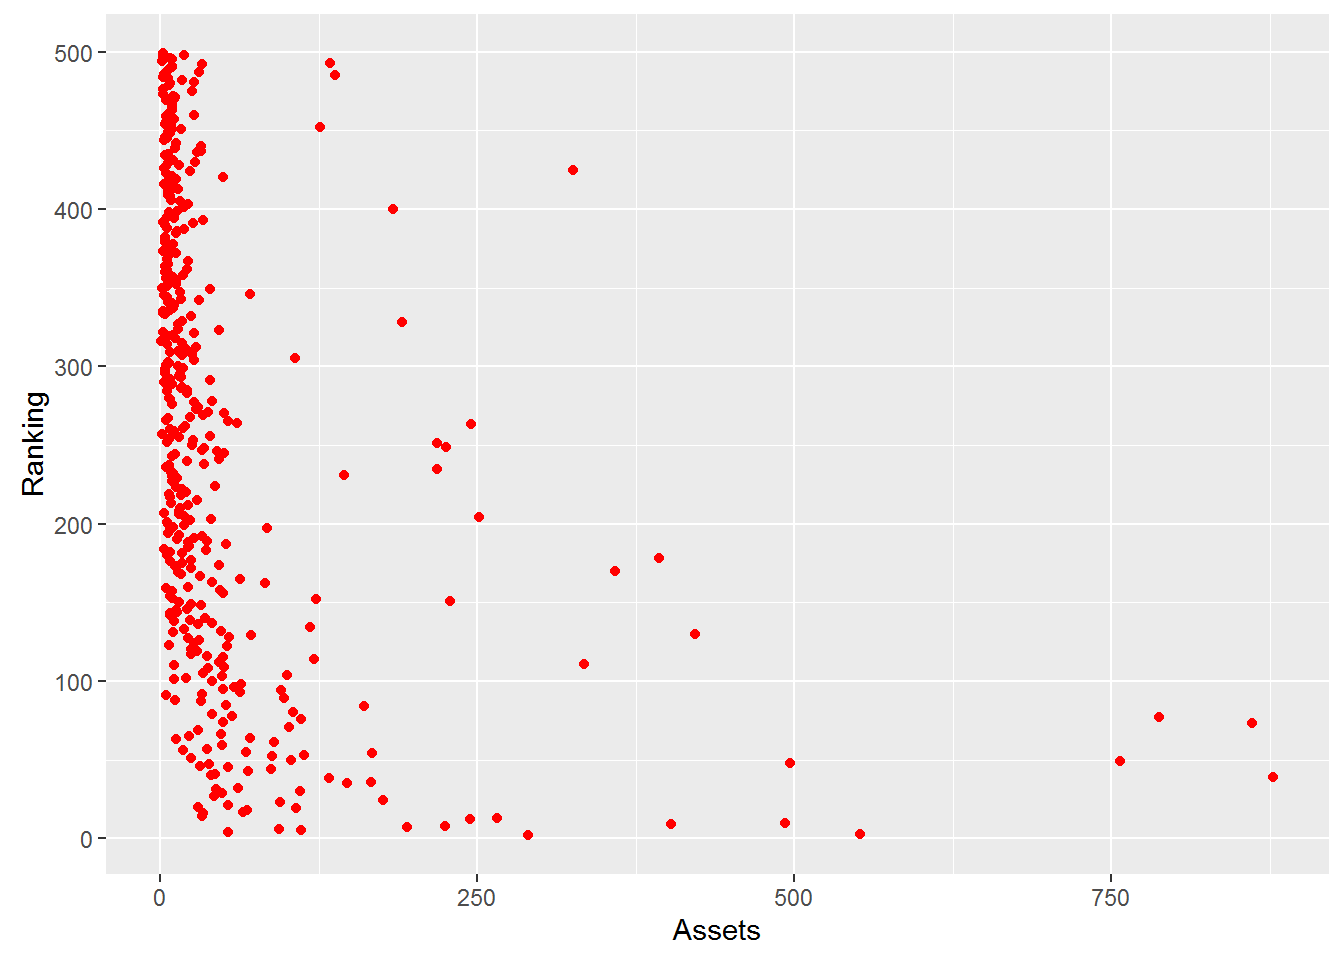
\includegraphics[scale=0.5]{../R/photos/05_rank_assets.png}  \\
\textit{We can see that there is no specific pattern that goes along with the Ranking here. Most companies have Assets until 100 million dollars.}
\end{center}
\end{table}

\begin{table}[H]
\centering
\caption{Market Value vs Ranking}
\begin{center}
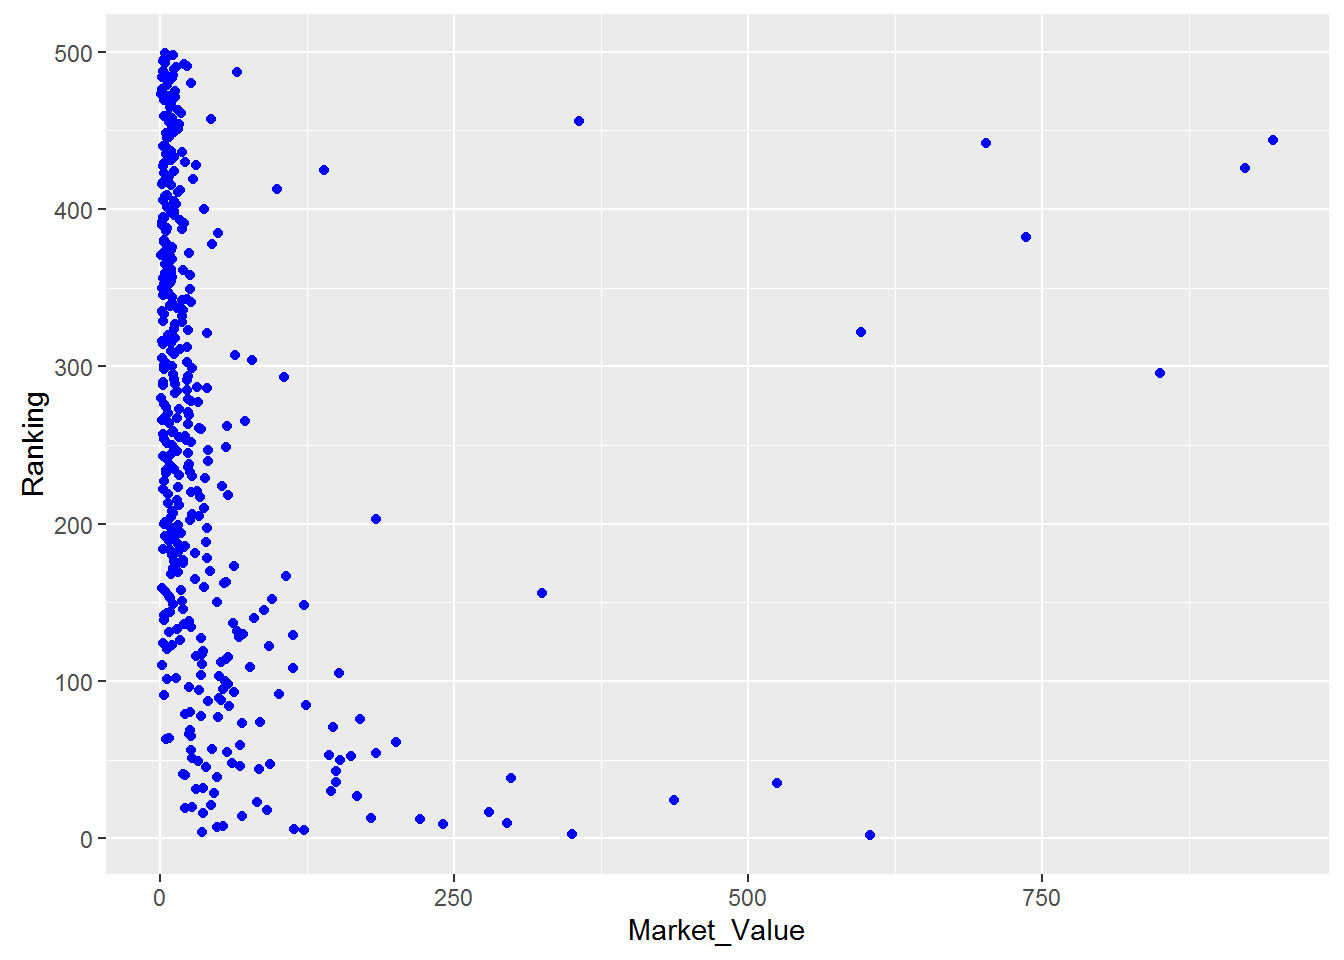
\includegraphics[scale=0.5]{../R/photos/06_rank_mark_val.png}   \\
\textit{Market value even though in the most high ranking (the lowest prices of ranking) shows a small differentiation and is bigger that in the lowest ranking still there is not a clear pattern.}
\end{center}
\end{table}

\begin{table}[H]
\centering
\caption{Total Stockholder Equity  vs Ranking}
\begin{center}
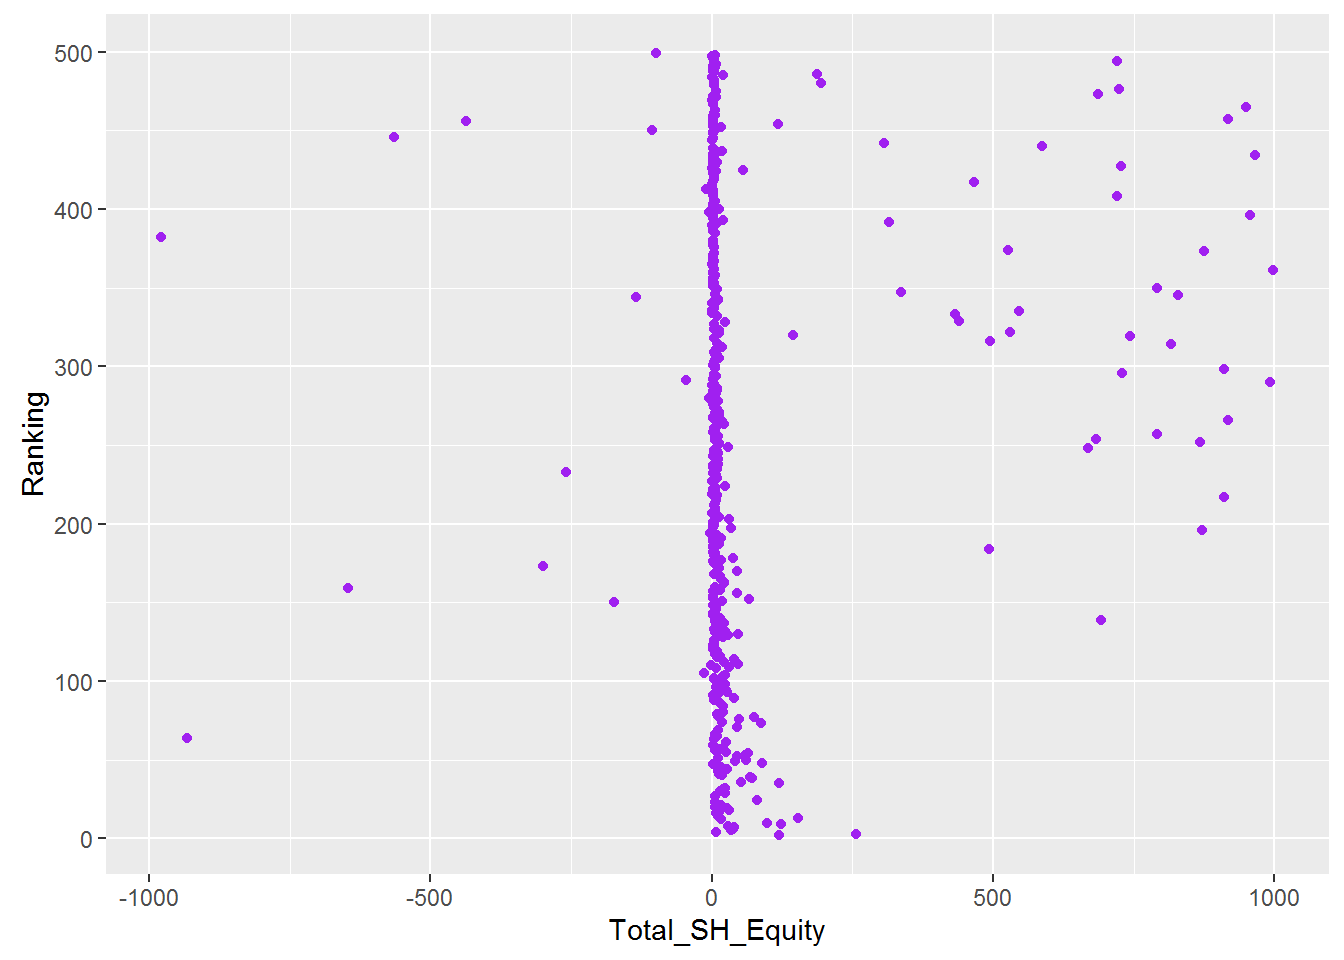
\includegraphics[scale=0.5]{../R/photos/07_rank_sh_eq.png}  \\
\textit{Most company total stockholder equity is until 50 million dollars but it does not change based on the Ranking.}
\end{center}
\end{table}

\begin{table}[H]
\centering
\caption{Revenues vs Ranking}
\begin{center}
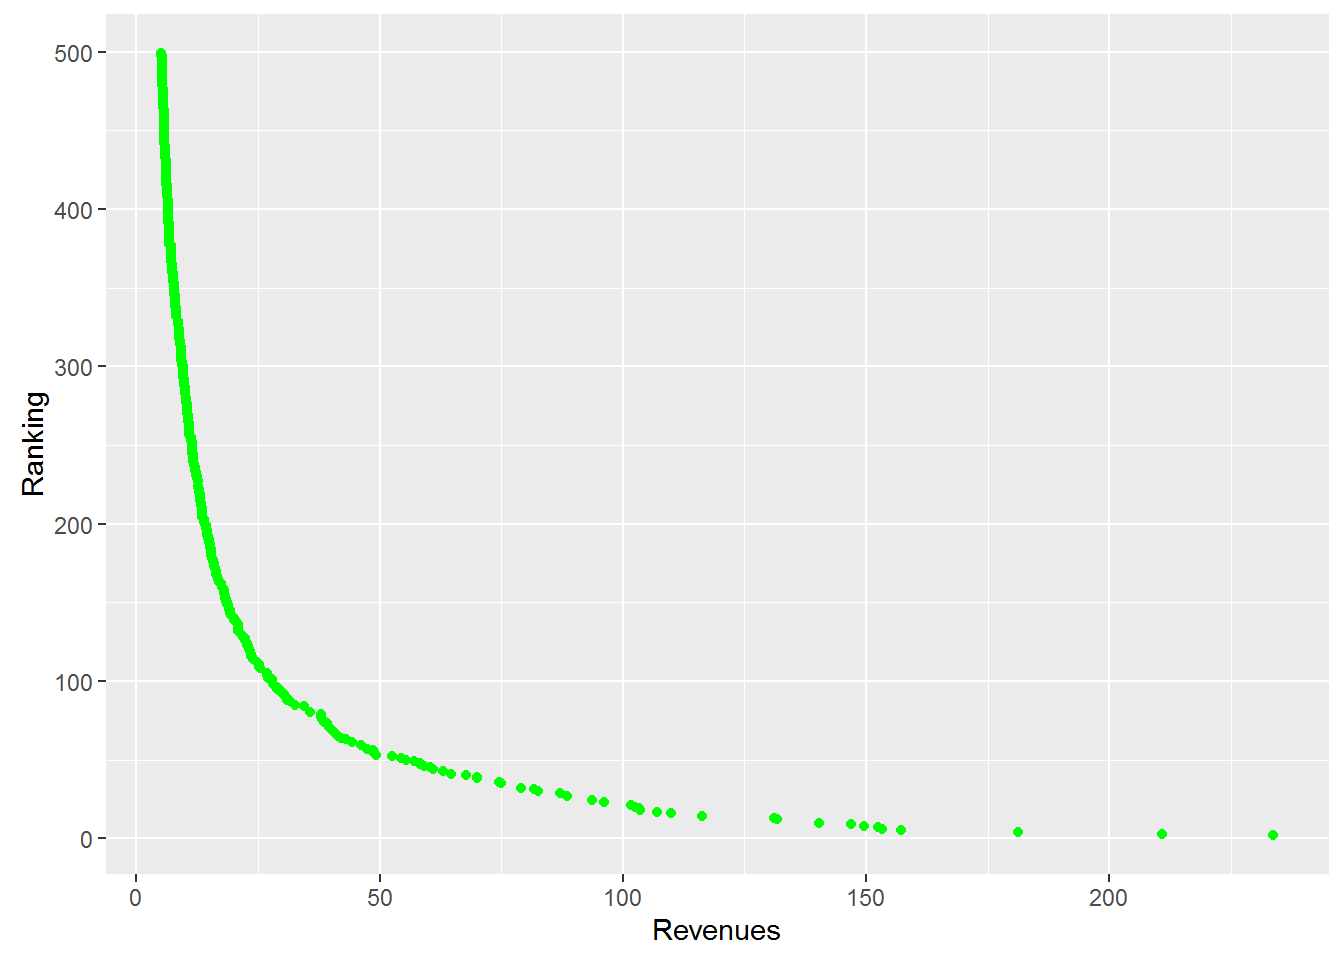
\includegraphics[scale=0.5]{../R/photos/08_rank_rev.png}  \\
\textit{As it was expected the smaller the Ranking (closer to top1 the bigger the Revenues. We can see a linear correlation between the two variables}
\end{center}
\end{table}

Based on the above diagrams we can conclude that the variable that we will use in order to see the influence of the websites variables in the company is the Revenues. As it is clear from the last diagram the Revenues have a linear correlation with the Ranking. The better the ranking the highest the Revenues so it is the ideal variable to see the actual success of each company in relation to the variables we have created. We can double check those finding with the help of the libraries corrplot and caret. We run a correlation plot with all the variables we have seen above:

\begin{table}[H]
\centering
\caption{Fortune variables correlation plot}
\begin{center}
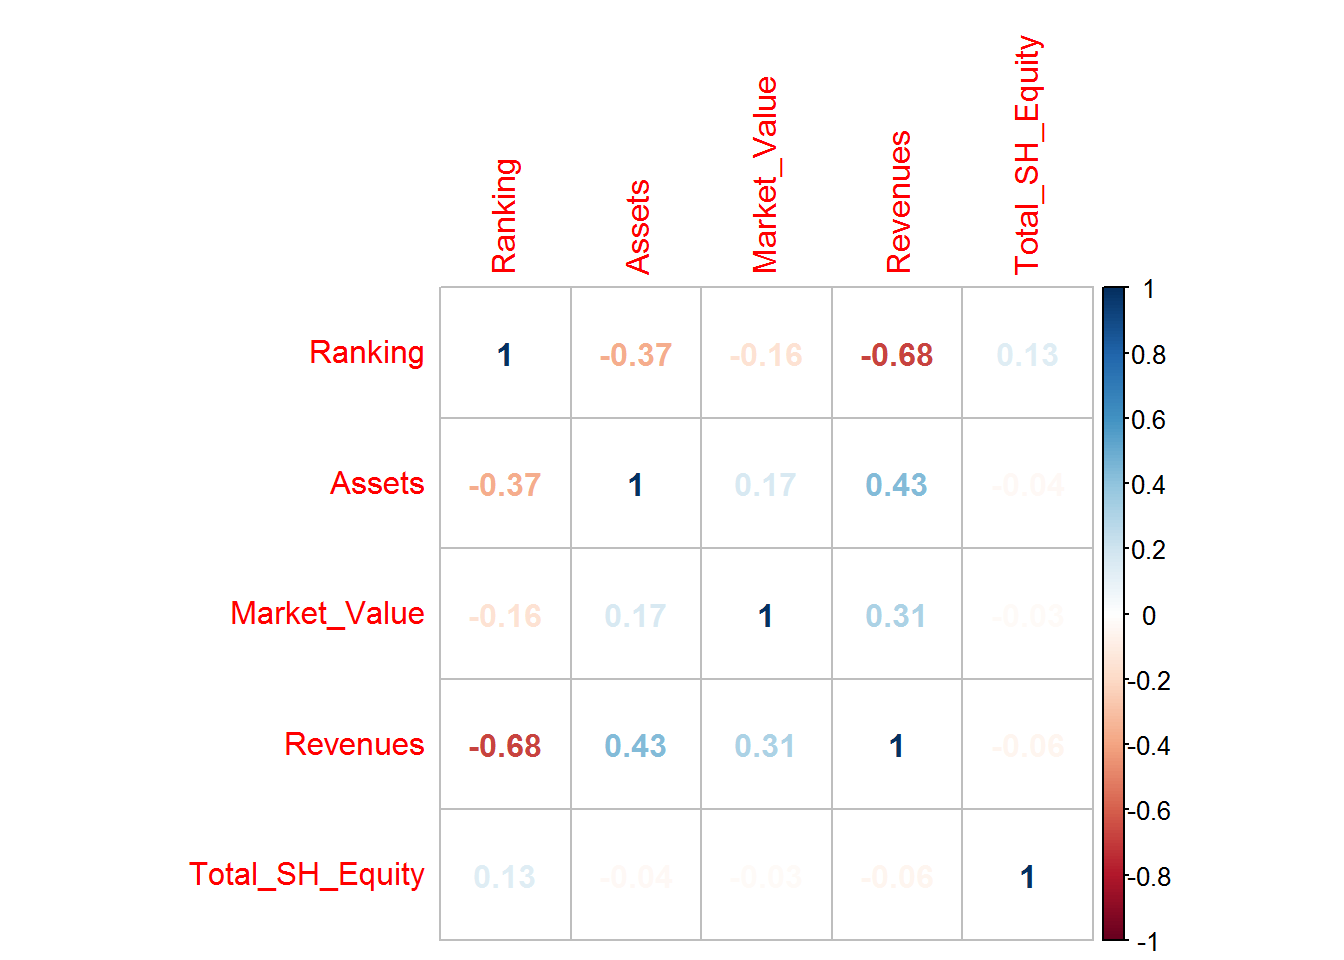
\includegraphics[scale=0.5]{../R/photos/09_rank_corplot_f500.png}   \\
\textit{From the chart we see that the strongest negative correlation is between Ranking and Revenues as we already have seen.}
\end{center}
\end{table}

Moreover the code that was used to create these diagrams is available in the Appendix.\ref{r: van: fortune}
\paragraph{Social media analysis and correlation}
Now that we have reach to the conclusion that the metric we will use from the Fortune 500 is the Revenues we will proceed with analysing the social media variables to see how they are distributed and then to see how they are correlated with the chosen variable.\\
\begin{table}[H]
\centering
\caption{Facebook}
\begin{center}
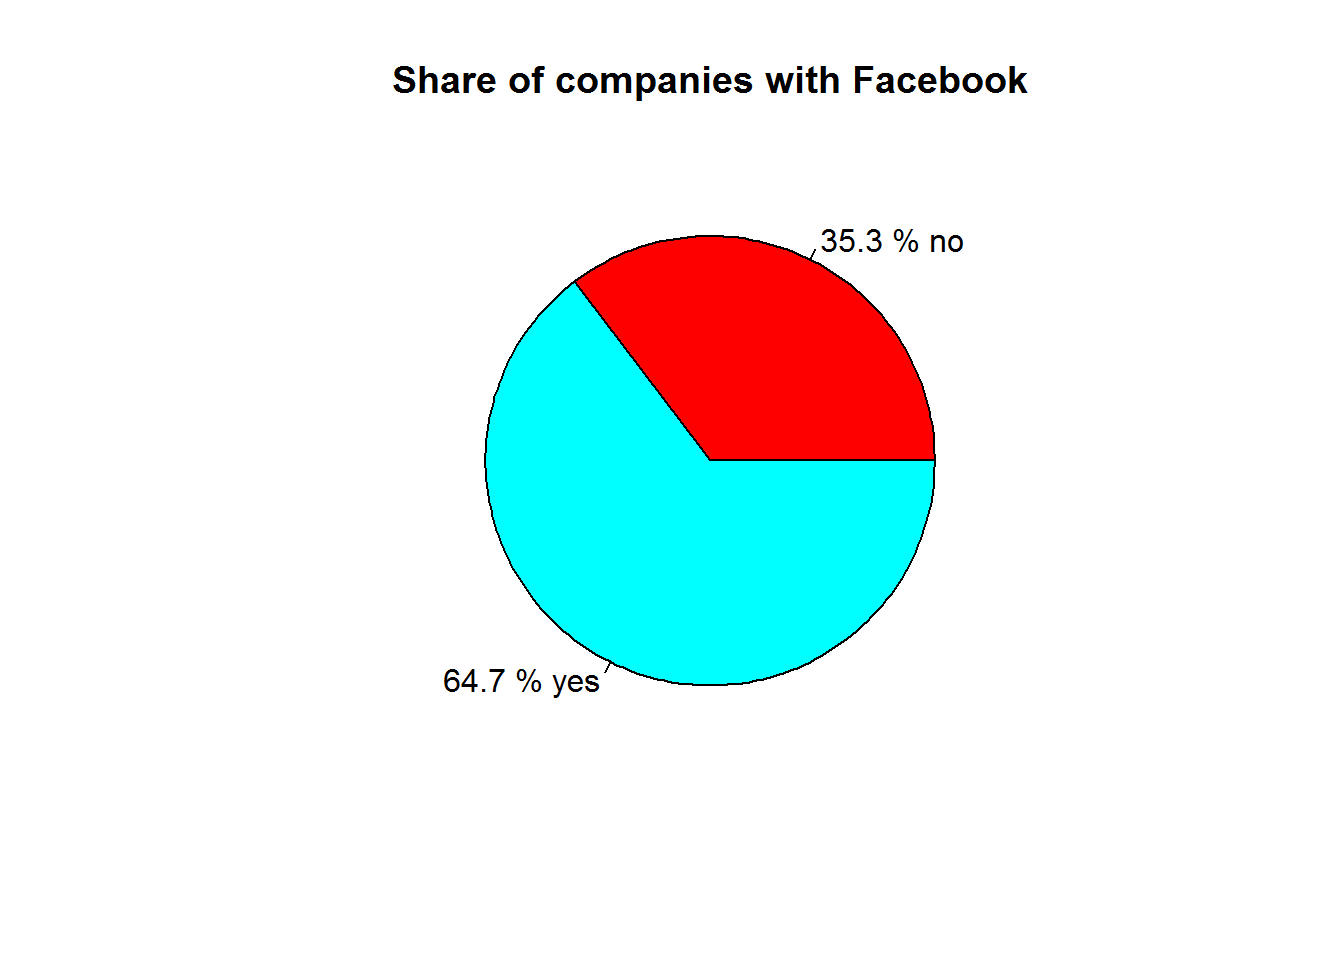
\includegraphics[scale=0.5]{../R/photos/10_facebook_dist.png}   \\
\textit{Almost the 65 percent of the companies that we are examining have Facebook links on their home page.}
\end{center}
\end{table}

\begin{table}[H]
\centering
\caption{Twitter}
\begin{center}
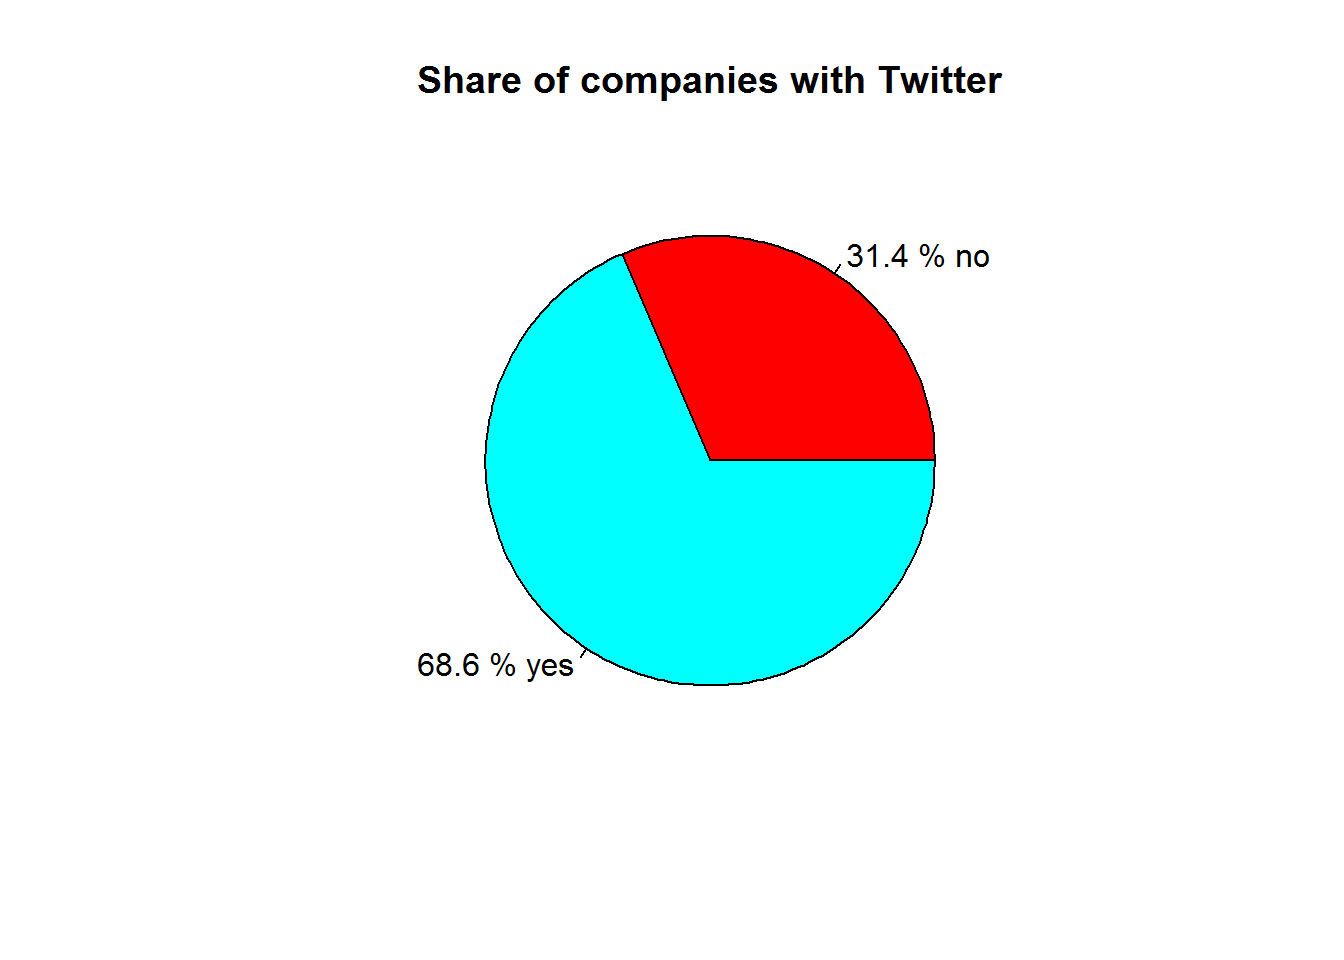
\includegraphics[scale=0.5]{../R/photos/12_tw_dist.png}  \\
\textit{Almost the 67 percent of the companies that we are examining have Twitter links on their home page.}
\end{center}
\end{table}

\begin{table}[H]
\centering
\caption{Instagram}
\begin{center}
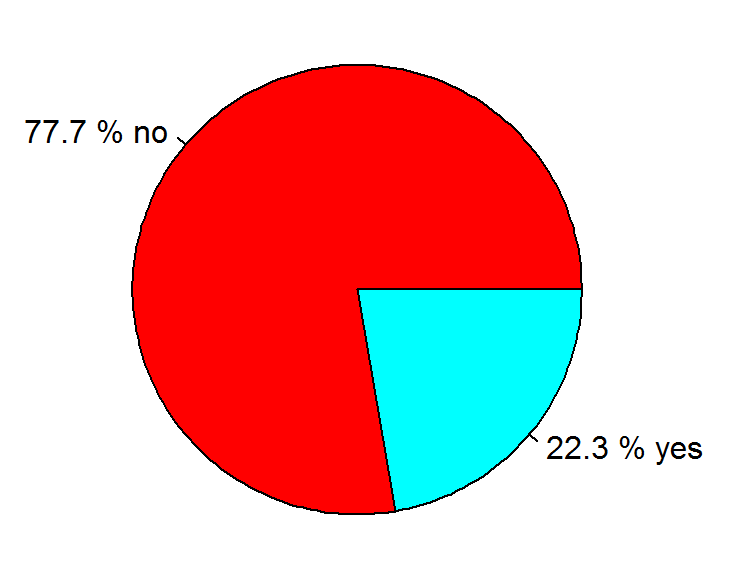
\includegraphics[scale=0.5]{../R/photos/14_inst_dist.png}  \\
\textit{Only the 22 percent of the companies that we are examining have instagram links on their home page.}
\end{center}
\end{table}

\begin{table}[H]
\centering
\caption{Pinterest}
\begin{center}
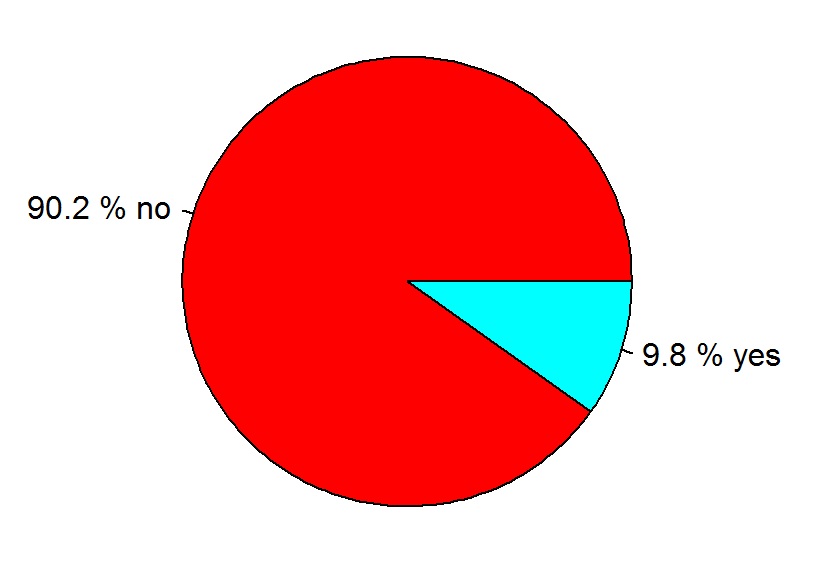
\includegraphics[scale=0.5]{../R/photos/16_pint_dist.png}  \\
\textit{Only a small 10 percent of the companies that we are examining have pinterest links on their home page.}
\end{center}
\end{table}

\begin{table}[H]
\centering
\caption{YouTube}
\begin{center}
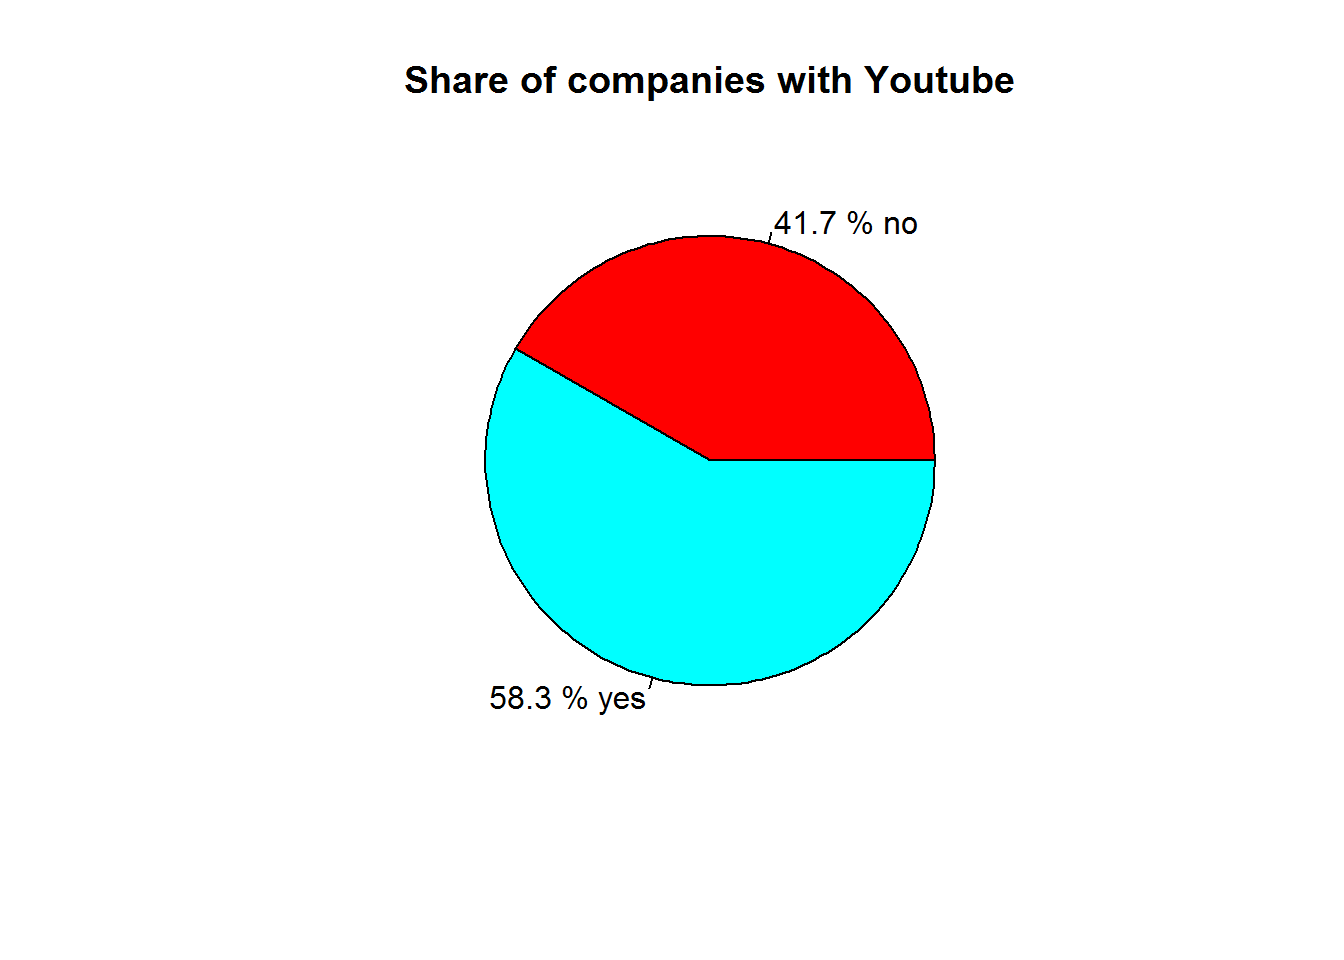
\includegraphics[scale=0.5]{../R/photos/18_yt_dist.png}  \\
\textit{The 58 percent of the companies that we are examining have YouTube links on their home page.}
\end{center}
\end{table}

\begin{table}[H]
\centering
\caption{LinkedIn}
\begin{center}
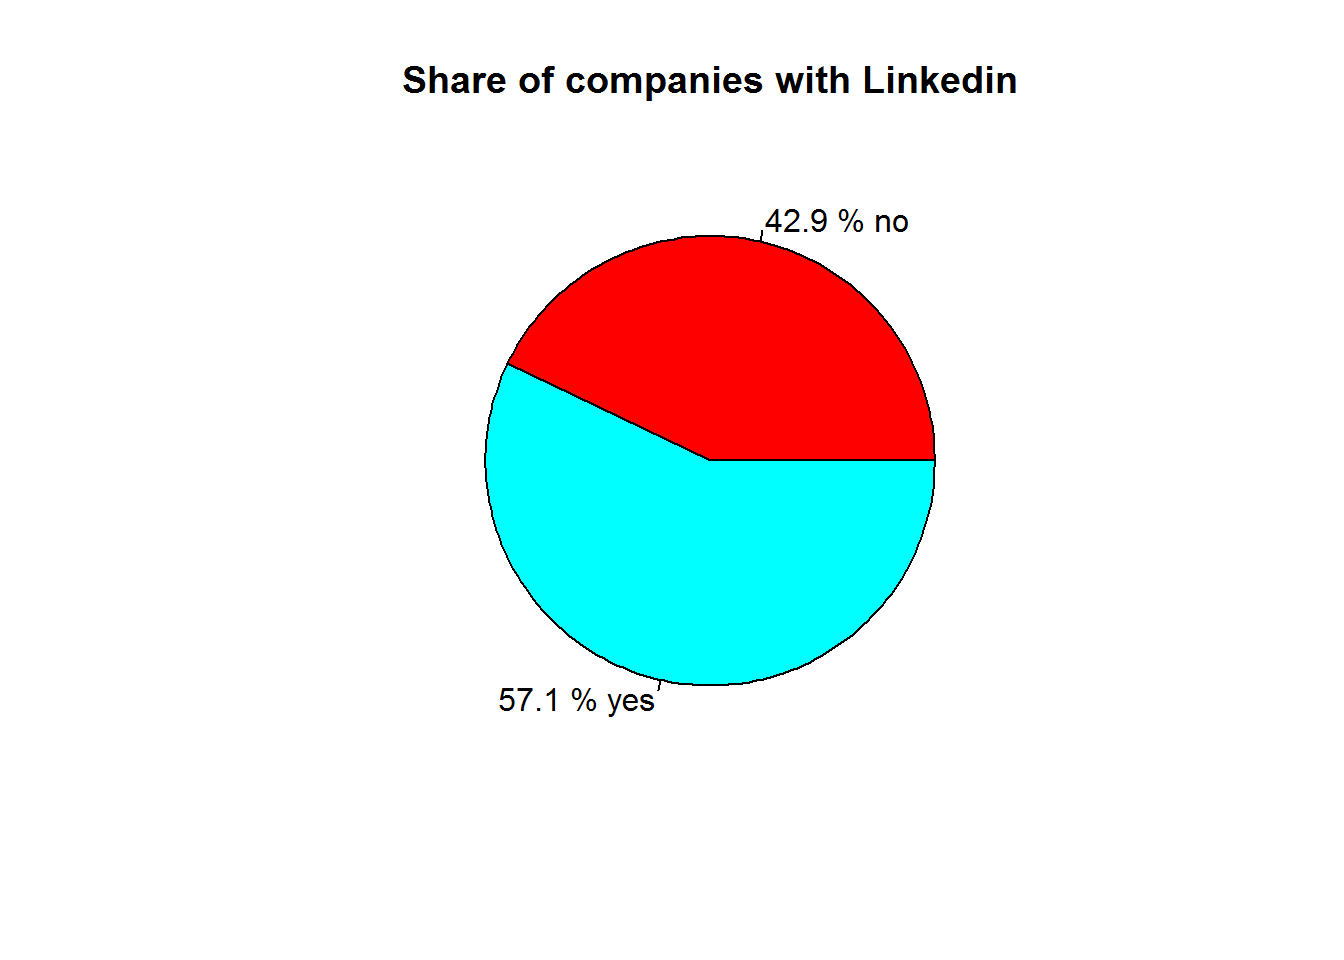
\includegraphics[scale=0.5]{../R/photos/20_linkedin_dist.png}  \\
\textit{The 57 percent of the companies that we are examining have YouTube links on their home page.}
\end{center}
\end{table}
From the above pie charts we can conclude that the most frequently used social media is Facebook and Twitter and the least used ones is Instagram and Pinterest. The first conclusion can be easily confirmed since those two first social media are the most widely known. Nevertheless instagram is being used from a great majority of people and many companies use it for campaigns.\\
The next step is to create a correlation chart with all the social media and the Ranking variable so as to see their relation:

\begin{table}[H]
\centering
\caption{Social media correlation}
\begin{center}
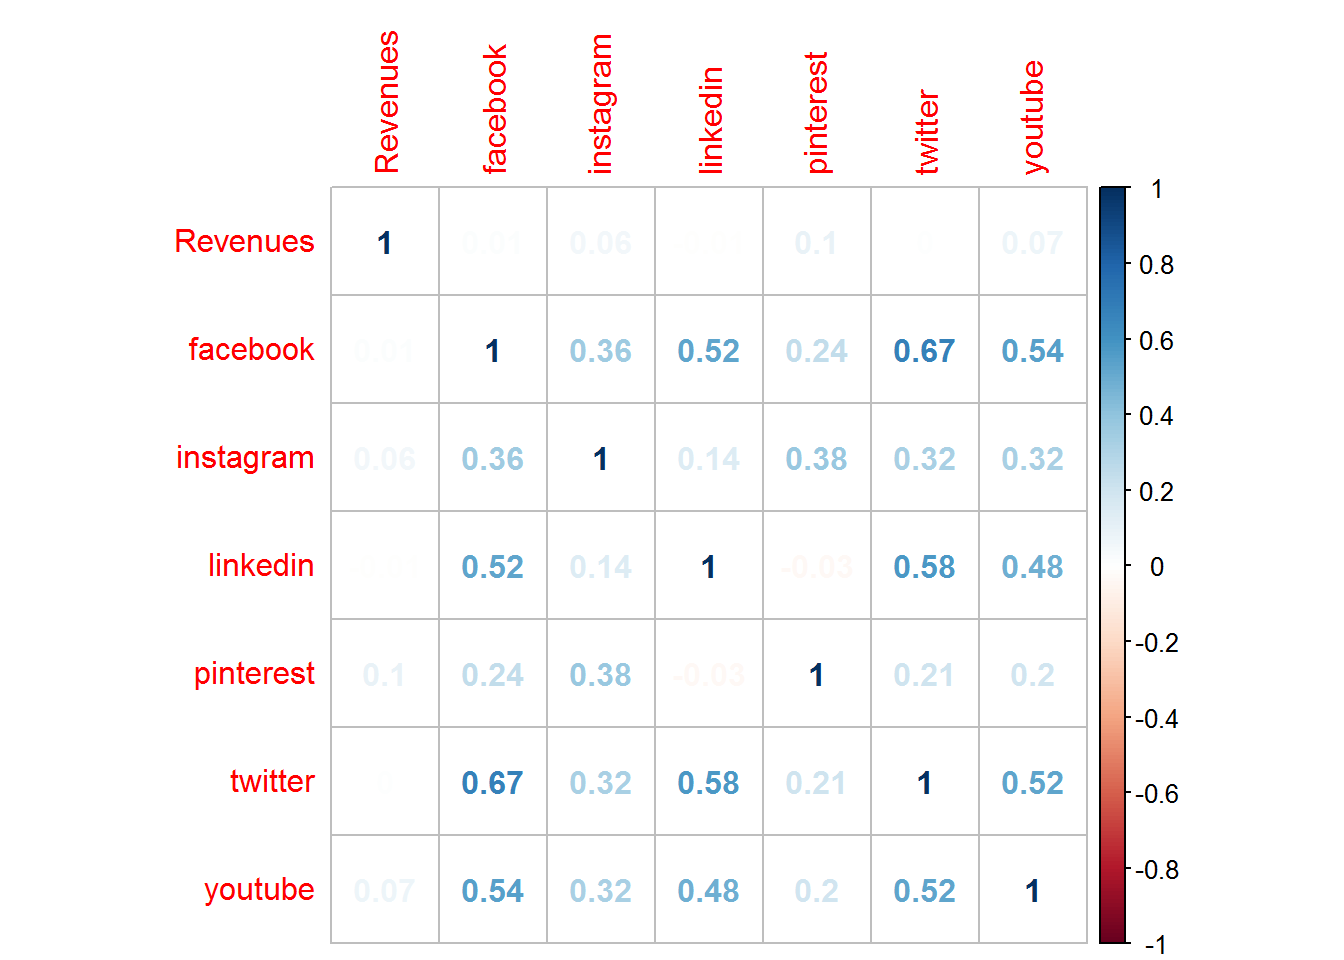
\includegraphics[scale=0.5]{../R/photos/22_REV_SM.png}  \\
\textit{Facebook has correlation more than 50 percent with twitter, youtube and linkedin and that the smallest correlations are those of pinterest and instagram.}
\end{center}
\end{table}

The same conclusions can derive from the correlation plot as well. The code we used to create those charts is available in the Appendix.\ref{r: van: sm}
\paragraph{Links analysis and correlations}
Next step is to analyse the distribution of the internal, external and total links and of course their correlation with each other and with the Revenues. We begin with the distribution of the variables in correlation with the Revenue variable:

\begin{table}[H]
\centering
\caption{Total Links}
\begin{center}
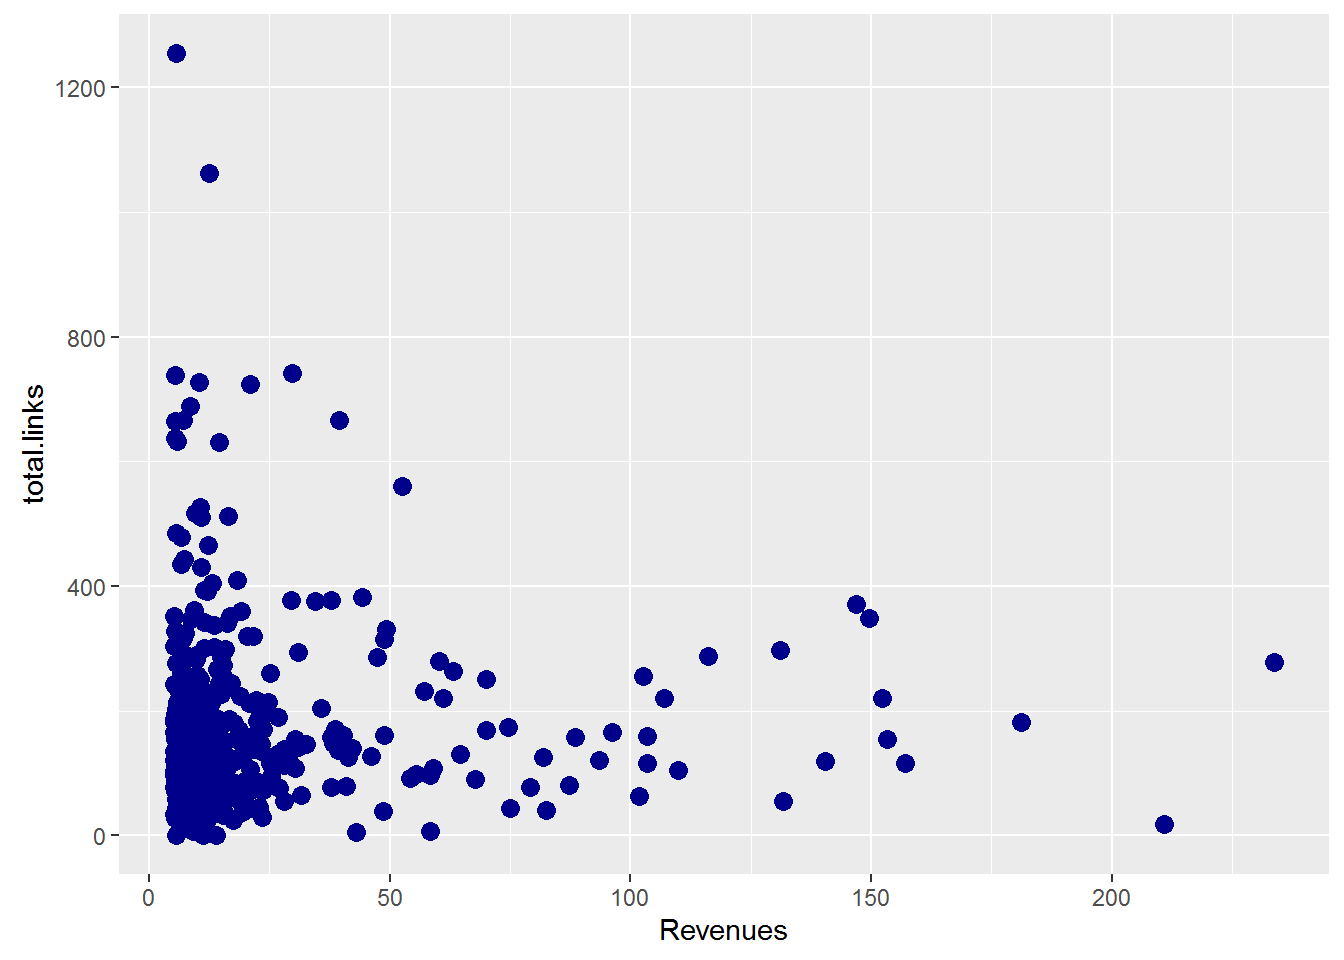
\includegraphics[scale=0.5]{../R/photos/24_totlinks_rev.png}  \\
\textit{We can see that as the Revenues increase the total links are steadily going under 400.}
\end{center}
\end{table}

\begin{table}[H]
\centering
\caption{External links}
\begin{center}
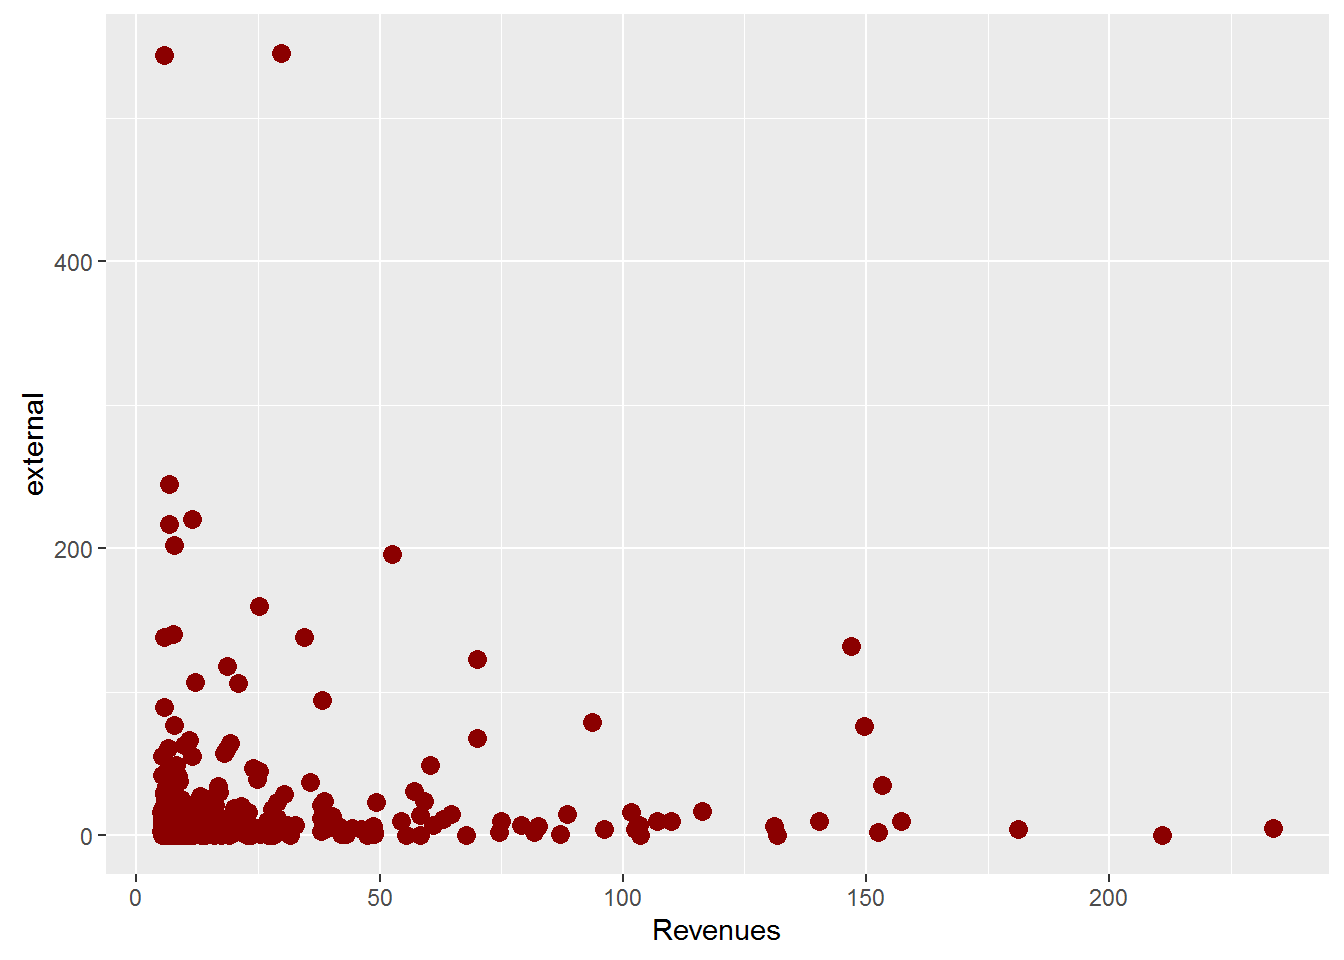
\includegraphics[scale=0.5]{../R/photos/26_ext_rev.png}  \\
\textit{Again as in the previous table as the Revenues increase the external links tend to go very low.}
\end{center}
\end{table}

\begin{table}[H]
\centering
\caption{Internal links}
\begin{center}
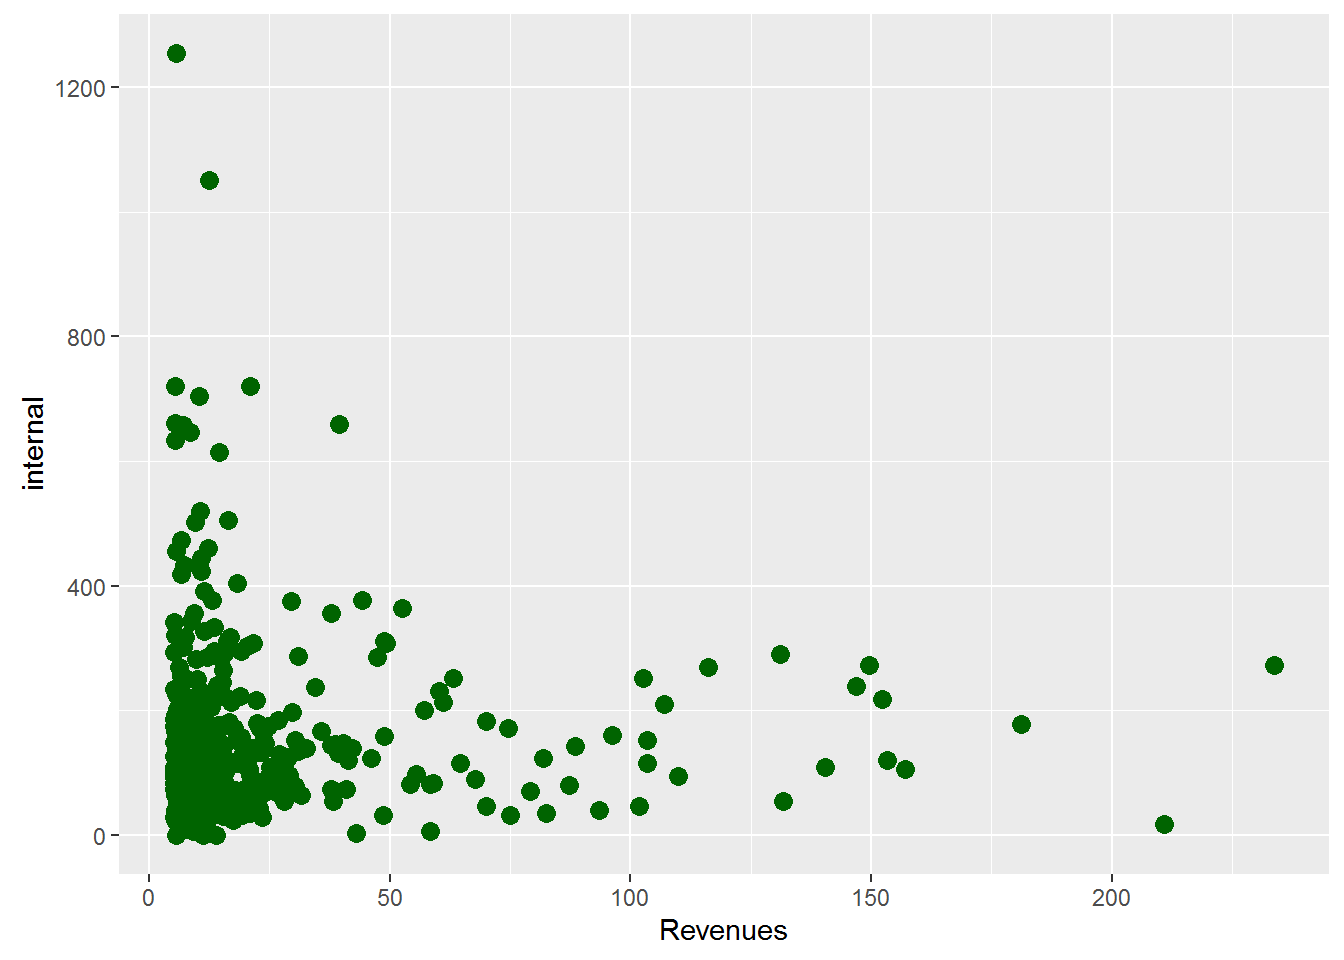
\includegraphics[scale=0.5]{../R/photos/28_int_rev.png}  \\
\textit{The internal links have a very similar distribution to the total links which is logical since the one is a subset of the other.}
\end{center}
\end{table}

Now that we have the first glimpse of the variables and we understand that when the Revenues are increasing the number of the link is under some specific margins we can create also the correlation table to see if we can extract any other useful information:

\begin{table}[H]
\centering
\caption{Links correlation table}
\begin{center}
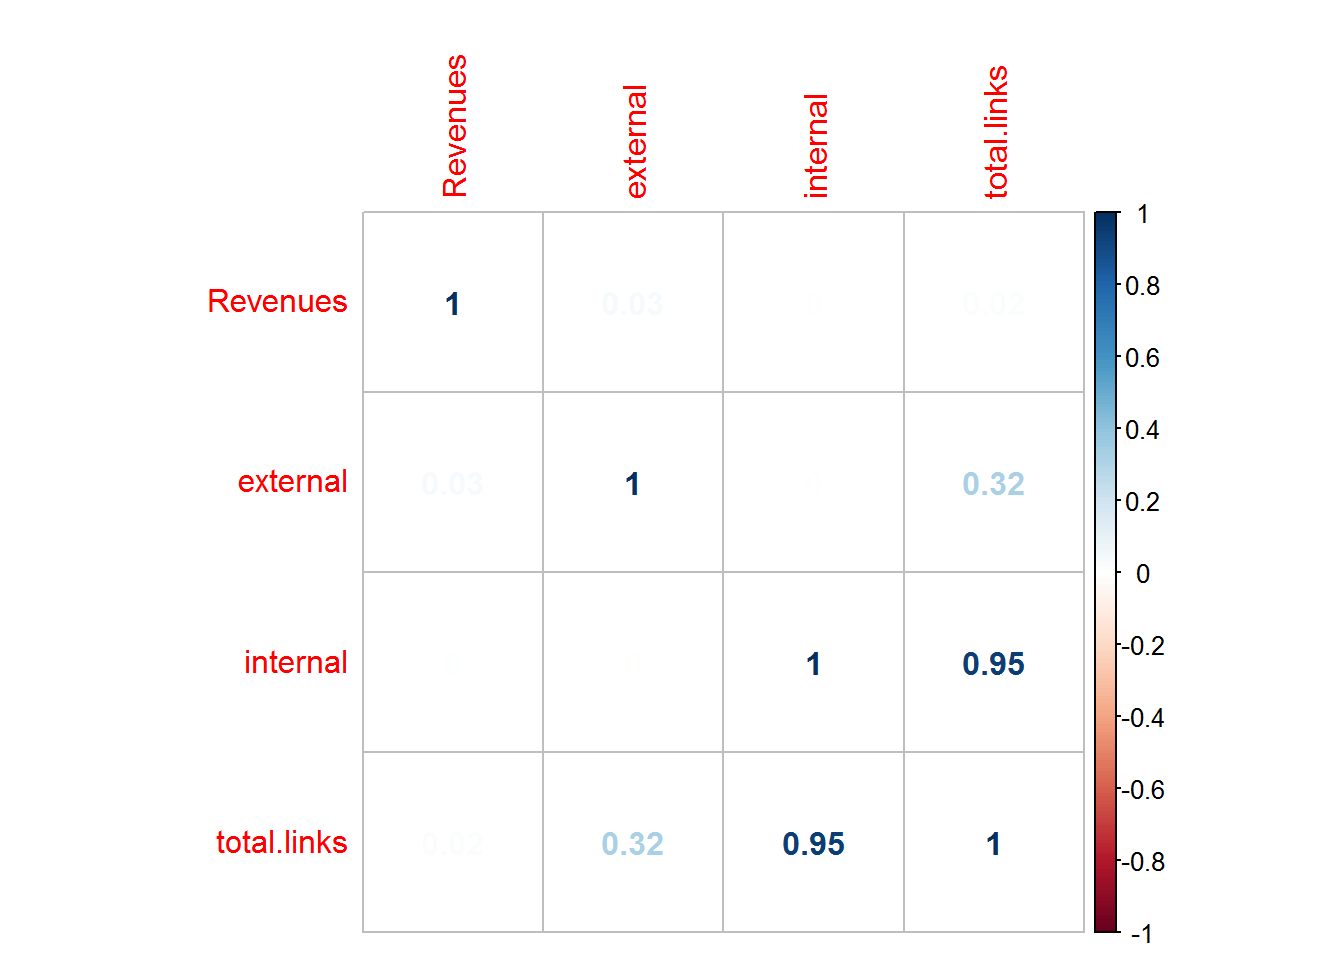
\includegraphics[scale=0.5]{../R/photos/29_rev_cor_links.png}  \\
\textit{The internal links are extremely correlated with the total links.}
\end{center}
\end{table}
From the correlation table we can see that the observation we made based on the previous charts, that the internal links distribution in relation to the Revenues is very similar to the one of the total links, can also be supported from this table were the correlation between the 2 variables is 95\%. This information might come handy later on when we are going to create regression models. The code for this section is available in the Appendix.\ref{r: van: l}
\paragraph{Loading time analysis and correlation}
The loading time of the sites is a very important key performance indicator usually in website performance so it is very interesting to see if it has any strong correlation with the Revenues of these very successful companies that we are examining.:
\begin{table}[H]
\centering
\caption{Loading time}
\begin{center}
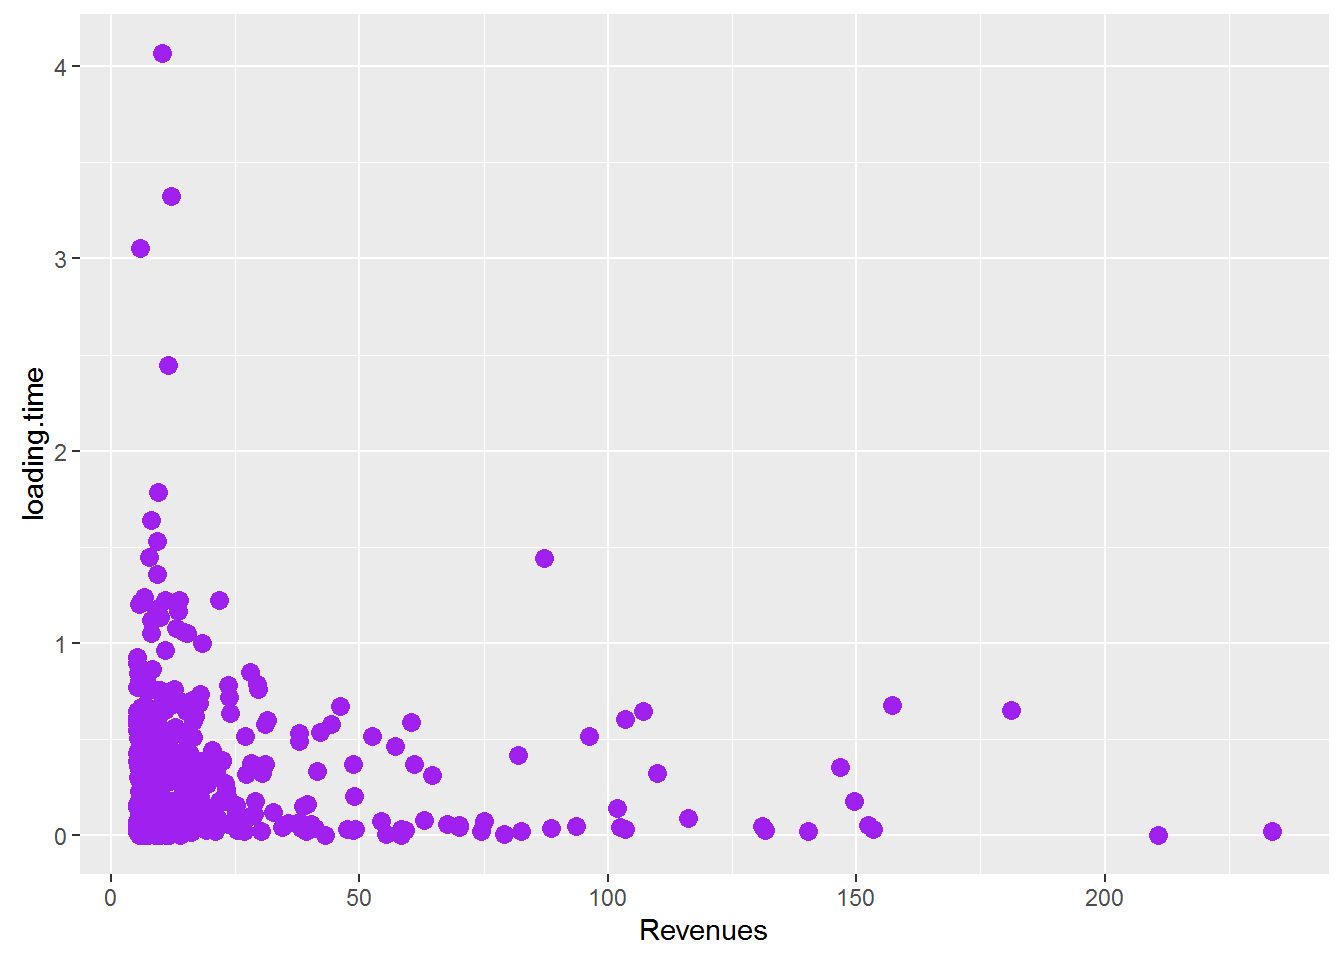
\includegraphics[scale=0.5]{../R/photos/31_ld_rev.png}  \\
\textit{Low loading time in the sites with the most Revenues.}
\end{center}
\end{table}
From the table above we can see that the loading time in relation to the Revenues has a small correlation. The companies that have the highest Revenues have also a very small loading time. Moreover we can see that the companies that have more than 100 million Revenues have loading times under 1 second. This observation shows that maybe the loading time is in fact a very important factor regarding the success of a website and moreover of a company overall success. The code for this table is available in the Appendix.\ref{r: van: load}
\paragraph{Content analysis and correlation}
The next step is to analyse the distribution of the variables that are related to the content and the text of the websites in relation to the Revenues of the companies at hand. As we explained in the Python chapter\ref{M:Content} we gathered 3 variables that are related to the grammatical overview of the text that is being used in the sites - which are the numbers of words, the number of unique words and the number of sentences - and 2 variables that are trying to explain if the content of this text is comprehensible from the majority of the users or not. Following below we have the charts with the distribution of those variables prices across the sites under examination and their relation to the Revenues.
\begin{table}[H]
\centering
\caption{Number of Sentences vs Revenues}
\begin{center}
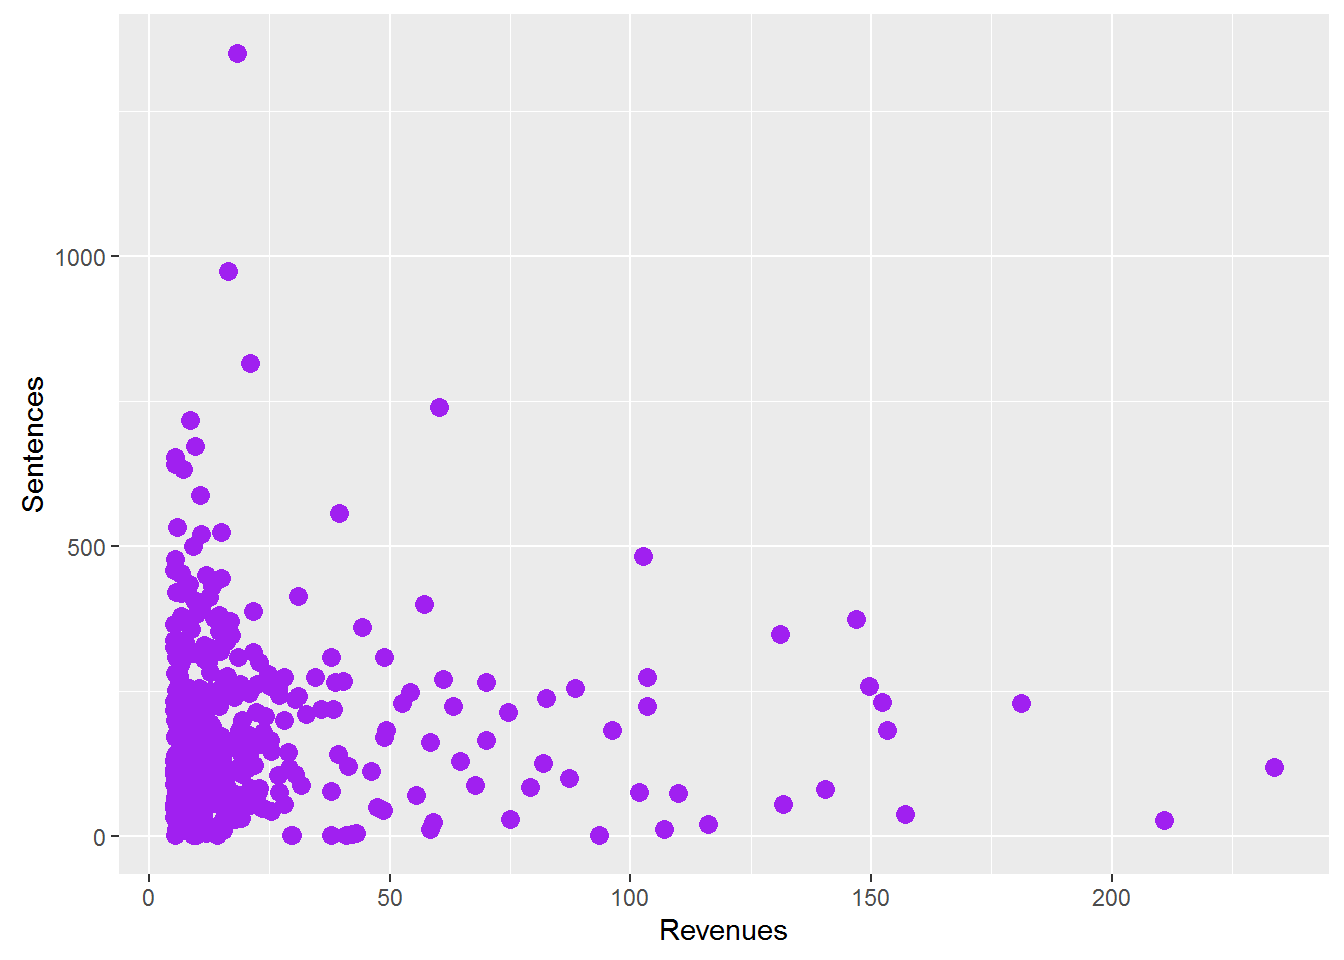
\includegraphics[scale=0.5]{../R/photos/33_sent_rev.png}  \\
\textit{In high Revenues the number of sentences is smaller that 500.}
\end{center}
\end{table}
From the table we can see that most sites have less than 500 sentences in their home page. Moreover while the Revenues price is going up the number of sentences seems to getting lower. For the sites that have more than 100 million dollars in Revenues the number of sentences drops under 250. Half the number of sentences that we can see in sites with lower Revenues.
\begin{table}[H]
\centering
\caption{Number of Words vs Revenues}
\begin{center}
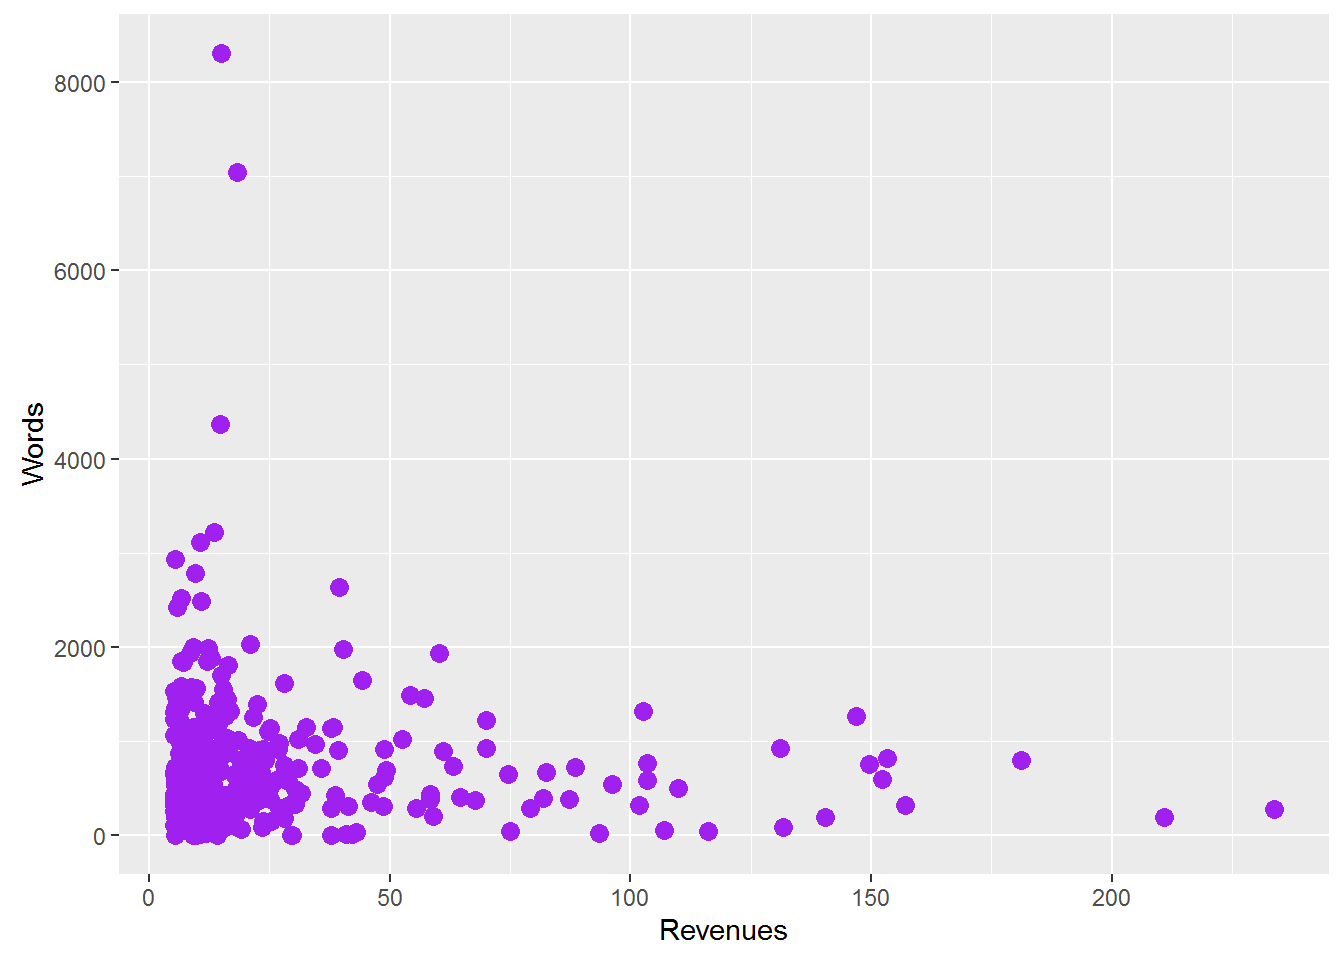
\includegraphics[scale=0.5]{../R/photos/37_w_rev.png}   \\
\textit{In high Revenues the number of words is smaller that 1000.}
\end{center}
\end{table}
By the same logic as the sentences in relation to the revenues so does the number of words seems to drop when the revenues go up. Furthermore here we can see that the decrease starts in lower revenues prices (around the 50 million dollars). This is expected if we take under consideration that the number of words is always correlated to the number of sentences. Most sites do not want to have very long sentences in order not to bore the reader. So since the number of sentences incline when the revenues are increasing we anticipate that the number of words will have the same reaction to the revenues.
\begin{table}[H]
\centering
\caption{Number of Unique Words vs Revenues}
\begin{center}
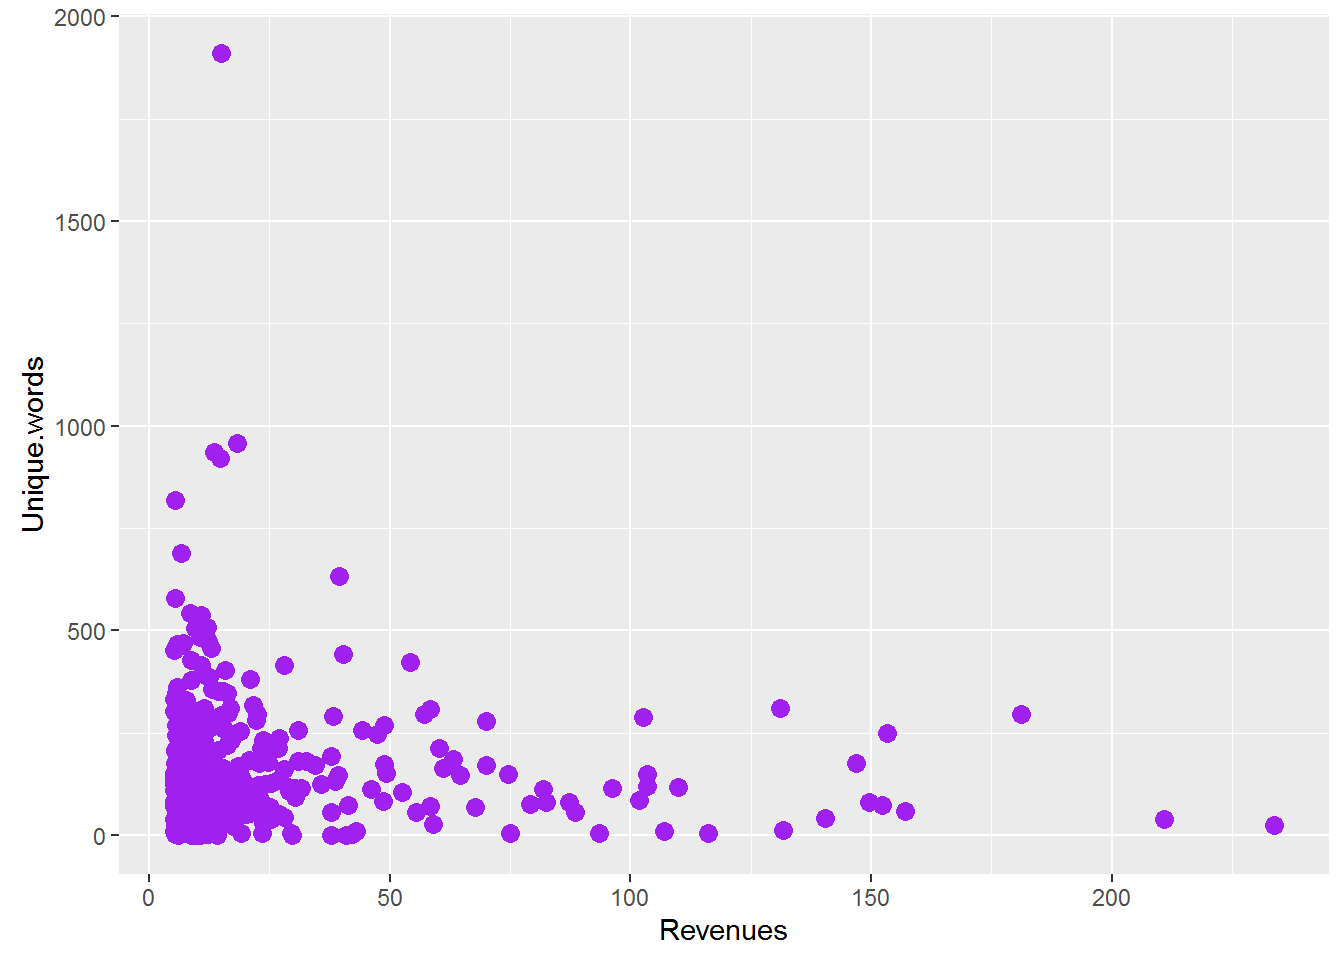
\includegraphics[scale=0.5]{../R/photos/35_uw_rev.png}    \\
\textit{In high Revenues the number of unique words is close to zero.}
\end{center}
\end{table}
The number of unique words differs from the actual number of all the words. Here we are trying to see how many not commonly used words does each site uses. Here the distribution is not so clear as it was for the two previous variables but still we can see that in the most sites that have high Revenues the number of unique words are very small. 
\begin{table}[H]
\centering
\caption{Correlation table}
\begin{center}
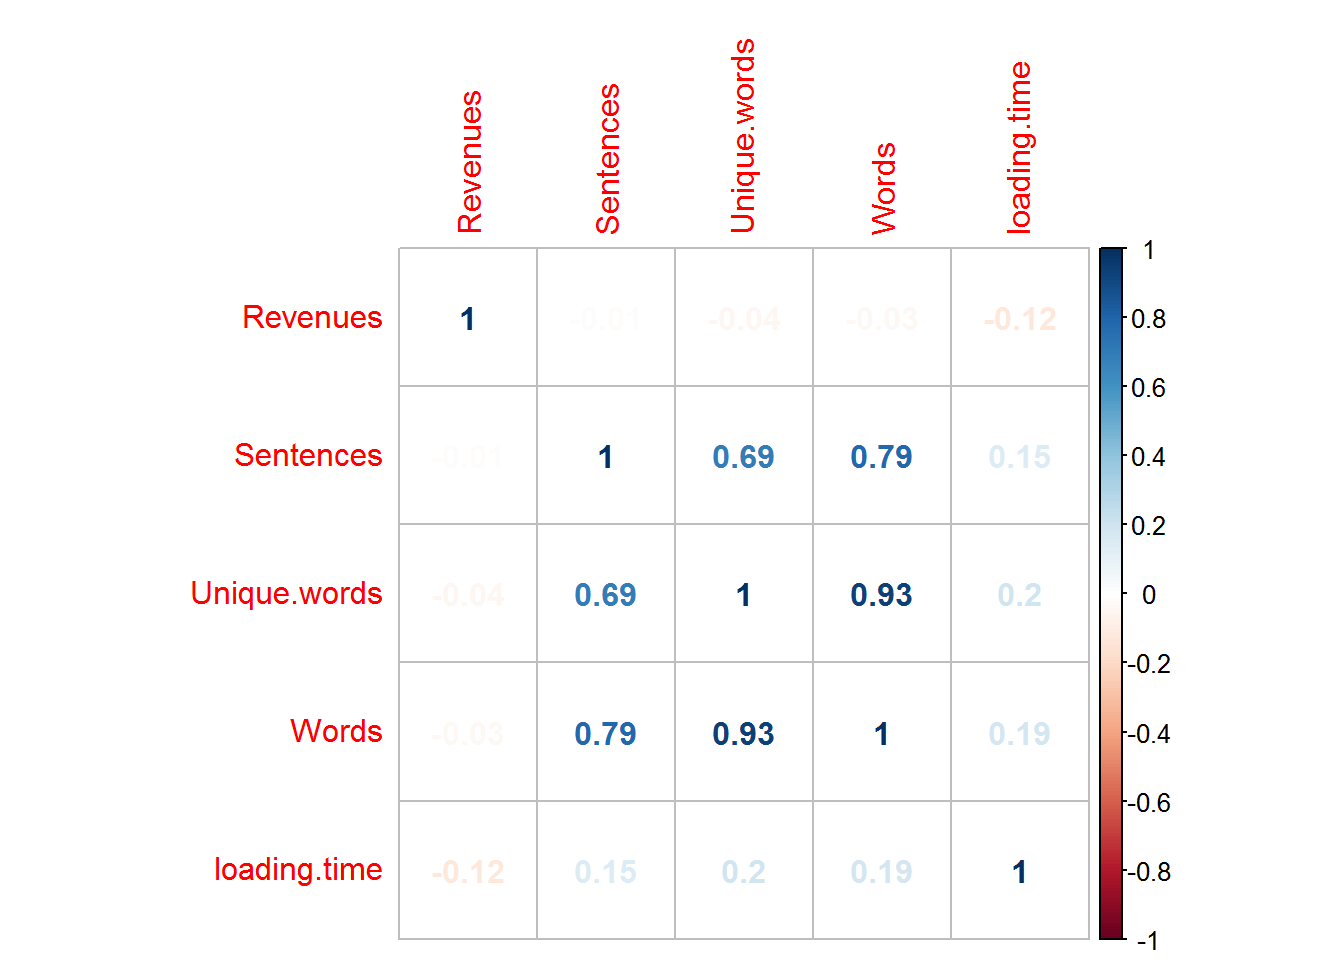
\includegraphics[scale=0.5]{../R/photos/38_words_corr.png}    \\
\textit{Sentences, words and unique words are highly correlated.}
\end{center}
\end{table}
From the correlation table we can also observe that the three variables we examined regarding the text of the websites are highly correlated with each other which as we already explained is an expected outcome.Moreover we can see that the Revenues with the loading time has a small negative correlation. This means that when the one variable price is going up the others' variable price should go down. This is also an expected outcome since as we said before the time a site does to open is very important to the users as they can easily grow impatient and look somewhere else. This is due to the grand variety of choices available on-line that makes the user feeling powerful.\\
Now that we analysed the 3 variables regarding the text attributes we should also analyse the 2 variables regarding the readability index of the websites' texts. Since of course the flesch measure variable was the source for calculating the readability variable we will analyse here only the readability variable thoroughly while the diagrammatically analysis of the flesh measure variable will be available in the Appendix.
\begin{table}[H]
\centering
\caption{Readability distribution table}
\begin{center}
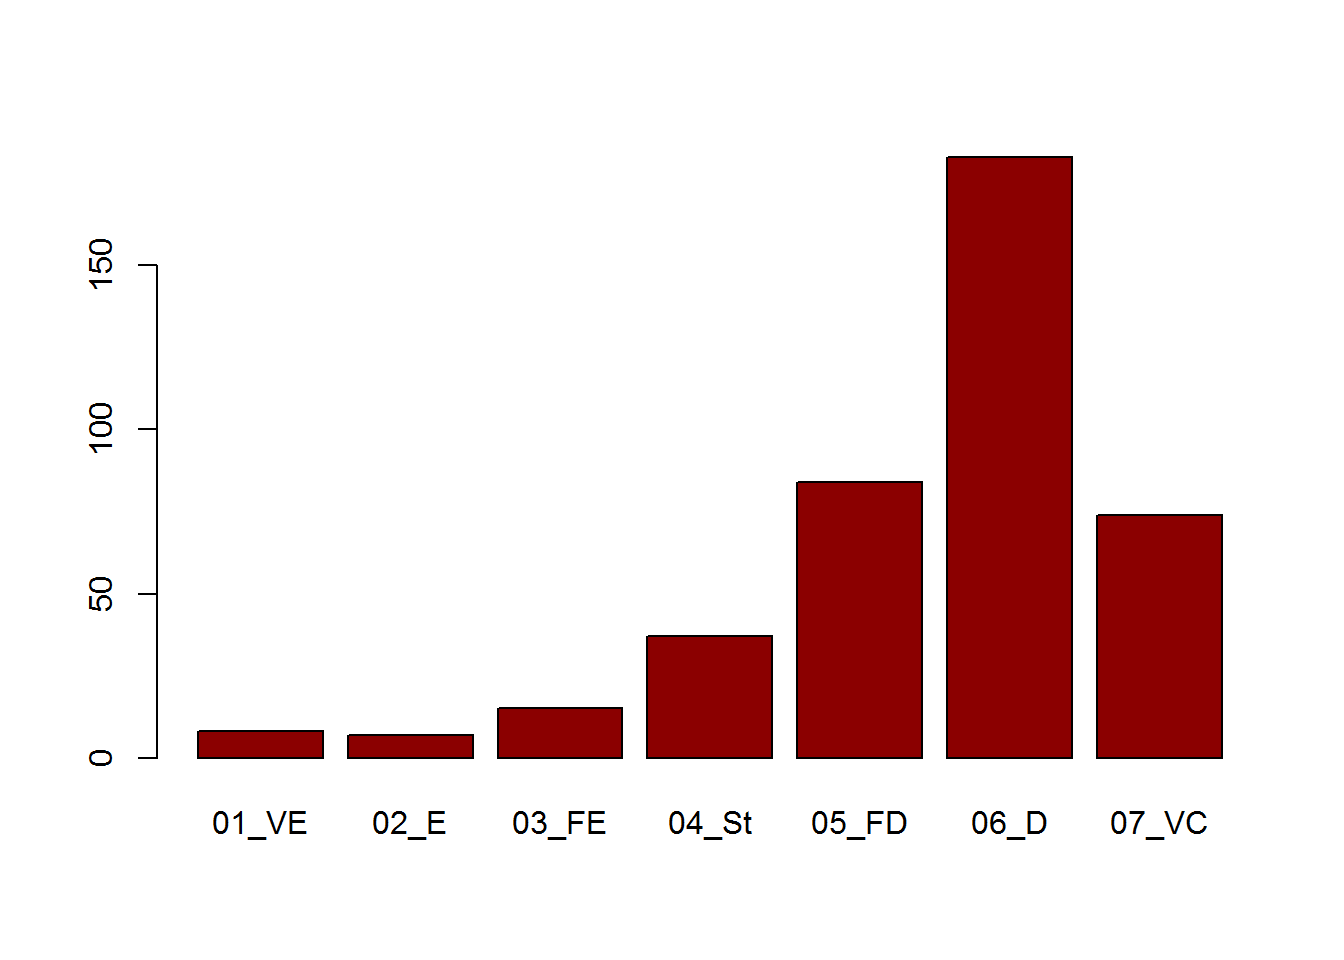
\includegraphics[scale=0.5]{../R/photos/41_read_dist.png}    \\
\textit{Most sites are difficult to read.}
\end{center}
\end{table}
\begin{table}[H]
\centering
\caption{Readability vs Revenues table}
\begin{center}
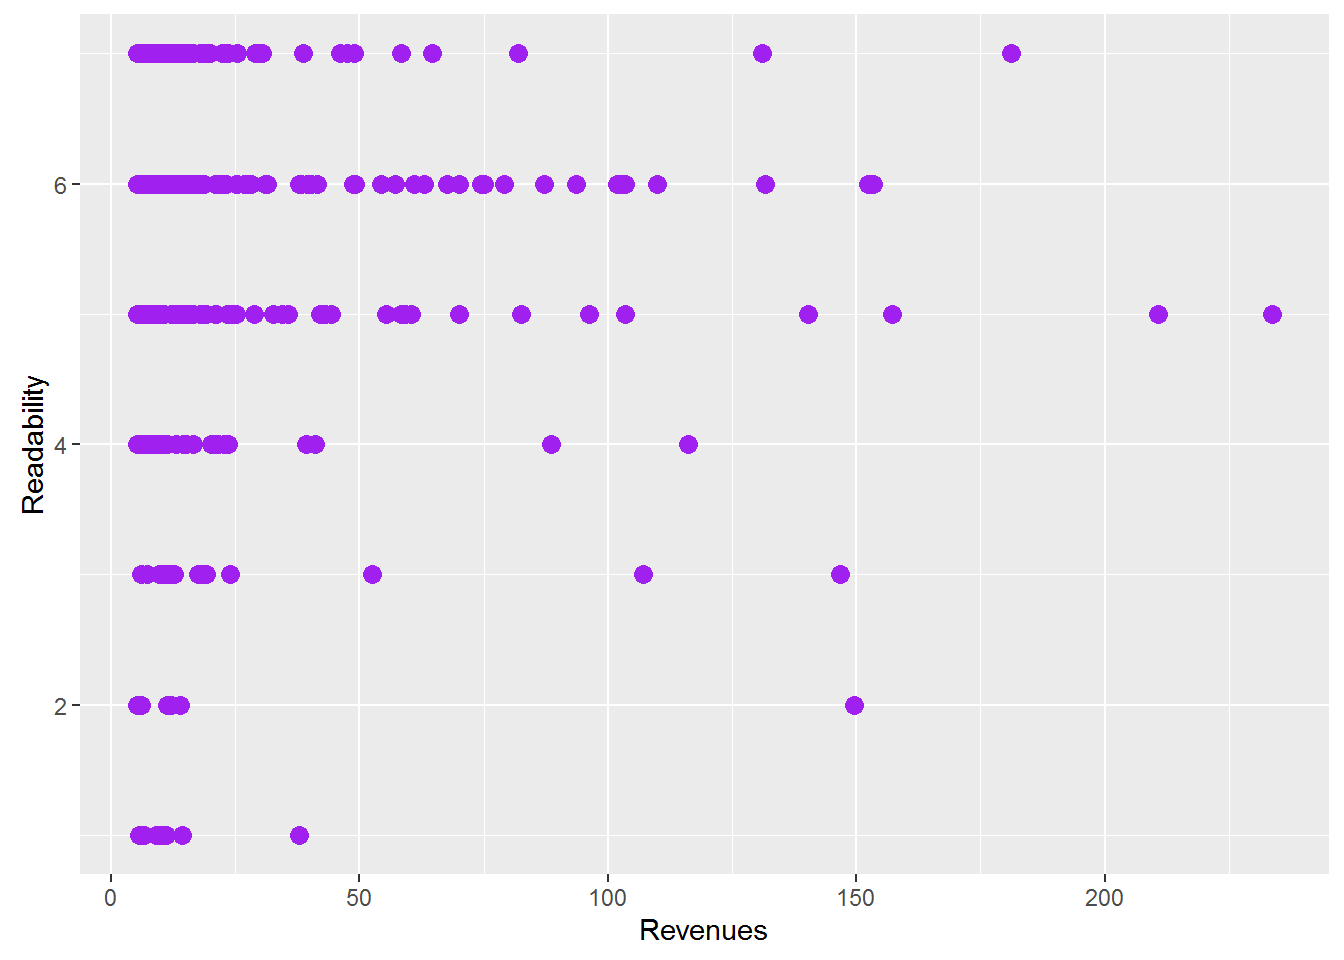
\includegraphics[scale=0.5]{../R/photos/42_read_rev.png}   \\
\textit{Most sites are difficult to read.}
\end{center}
\end{table}
From the above two charts we can see that firstly the most sites are difficult to be read and secondly that the readability index in relation to the Revenues does not show a clear pattern. The two sites with the most Revenues seems to be fairly difficult to read. What we can definitely see is that the sites that are very easy to be read all have revenues under 50 million dollars. This could mean that even though the users do not want to read very difficult texts they also do not want extremely easy ones. Maybe the correlation plot could help us have a clearer view of the relationship between the 2 variables.
\begin{table}[H]
\centering
\caption{Correlation table}
\begin{center}
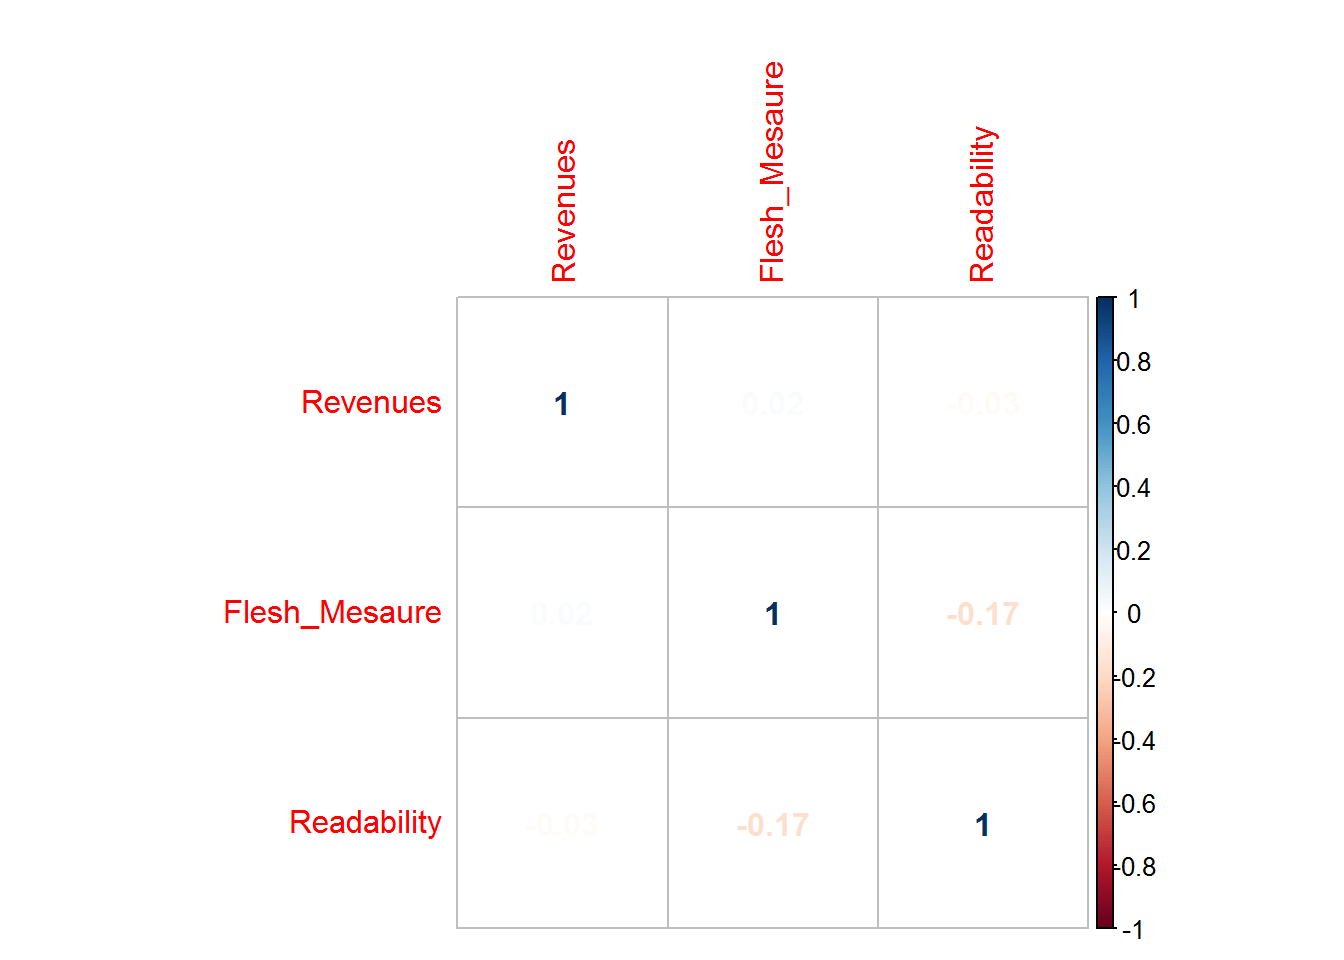
\includegraphics[scale=0.5]{../R/photos/43_read_cor.png}    \\
\textit{Flesh measure and readability variables are negative correlated.}
\end{center}
\end{table}
From the correlation plot we can see that the Revenues have a very small negative correlation with the readability variable. While the readability variable and the flesh measure variable as it was expected they have a negative correlation. This means that the bigger the price in the flesch measure the lower the price in the readability variable. If we consider that the best prices of the flesh measure are the highest while respectively for the readability variable are the lowest then it is a normal correlation.
\paragraph{HTML validation variables analysis and correlation}
During the extraction of the html validation variables we created 4 different metrics: the number of errors, the number of warnings the non document error and the page not opened one. In this chapter we are going to analyse the distributions of those variables and also their correlation with the Revenues.
\paragraph{Image types analysis and correlation}
Last but not least we should analyse the distribution of the different types of images that are being used on the websites that we are examining and also compare the total images with the Revenues to see the correlation.
\subsubsection{Data manipulation}
In this chapter we are going to change some of the variables that we have created in order to make them more easy to be analysed and explained in relationship to the Revenues. 
\paragraph{Image sizes variables reconstruction}
After implementing the python code for the size images (2.4.10) we created almost 700 different variables. This number is almost prohibited when it comes to regression models especially when the actual number of the examined cases are a lot fewer (500). That is why we decide to group this 700 variables to 5 new ones that we will be able to incorporate to this analysis.
\paragraph{Remove variables}
Now that we have created and analysed all the needed variables we can subtract from the data frame the variables that we have decide not to include in the regression analysis that will follow.
\subsubsection{Logistic Regression}
In this chapter we will perform logistic regression to the chosen data frame in order to determine the variables that affect most the price of the Revenues of a company
\paragraph{Training and test set creation}
Before we begin with the regression we have to divide the data frame to 2 data frames so as to be able to test the model we will create. We will make a training set and a test set.
\paragraph{Null and Full model creation}
The first step is by using the training set to create a null model (that includes only the Revenues) and a full model (that includes all the variables)
\paragraph{Lasso Method}
The next step is to implement the Lasso method
\paragraph{Both Method}
We will continue by applying the both method of the logistic regression in order to see if the variables that will be kept are the same or less than the lasso method.
\paragraph{Predictions and comparison of models}
Now we will make the predictions using the test set in order to compare how well do the model that we created work in practise.
\subsubsection{Comparisons and other methods}
Now that we have a first idea of the metrics that are considered more important it would be wise to use other methods to double check the results.
\paragraph{Correlation testing}
By seeing the correlations of the chosen variables we could create models by subtracting some of them to see if the results will be improved.
\paragraph{Clustering testing}
We will use the clustering method to see how the variables are being group together. And which variables play the most important role.
\paragraph{Final testing}
Now we will compare the results to see if we can test any other theory so as to be sure about the final results.
\paragraph{Final model}
After completing the analysis we can conclude that the most important variable of the websites that can play a crucial role to the actual revenues of a company are the images. More specifically the sizes and the type of the images along with the external links.
\pagebreak  
\section{Conclusions}
This conclusion can be easily explained from the fact that the eye is drowned to specific stimulations. There are many studies that shows that where the eye is going in the first seconds that a user is visiting a page can be crucial. So the right type of image with a correct structure and use of specific image sizes can make a site more likeable and friendly to the users.\\
Example - Testing of where does the eye drops first\\
Example - Images and the importance to the psychology\\
Example - Type of images more easily and rapid loading\\
Example - Information that the user is looking for not confined only inside the same website\\
\pagebreak  
\section{Bibliography}
\begin{thebibliography}{widest-label}

\bibitem{key1}$https://en.wikipedia.org/wiki/Fortune_500$
\bibitem{key2}$http://beta.fortune.com/fortune500$
\bibitem{key3}$http://www.tablesgenerator.com/$
\bibitem{key4}$https://www.continuum.io/downloads$
\bibitem{key5}$https://validator.w3.org/$
\bibitem{key6}Rui Miguel Forte,Mastering Predictive Analytics with R,Packt Publishing Ltd.,June 2015


\end{thebibliography}

\newpage
\appendix
\section{Appendix A: Fortune 500 Companies} \label{appA}
% the \\ insures the section title is centered below the phrase: AppendixA
\begin{table}[H]
\centering
\caption{Fortune 500 - Companies Ranked: 51 - 100}
\begin{tabular}{lll}
\hline
 & & \\
51. Intel
& 52. Humana
& 53. Disney
 \\ 
 54. Cisco Systems
& 55. Pfizer
& 56. Dow Chemical
 \\ 
57. Sysco
& 58. FedEx
& 59. Caterpillar
 \\ 
60. Lockheed Martin
& 61. N.Y. Life Insurance
& 62. Coca-Cola
 \\ 
63. HCA Holdings
& 64. Ingram Micro
& 65. Energy Transfer Equity
 \\ 
66. Tyson Foods
& 67. American Airlines Group
& 68. Delta Air Lines
 \\ 
69. Nationwide
& 70. Johnson Controls
& 71. Best Buy
 \\ 
72. Merck
& 73. Liberty Mutual I.G.
& 74. Goldman Sachs Group
 \\ 
75. Honeywell International
& 76. Massachusetts Mutual L.I.
& 77. Oracle
 \\ 
78. Morgan Stanley
& 79. Cigna
& 80. U.C. Holdings
 \\ 
81. Allstate
& 82. TIAA
& 83. INTL FCStone
 \\ 
84. CHS
& 85. American Express
& 86. Gilead Sciences
 \\ 
87. Publix Super Markets
& 88. General Dynamics
& 89. TJX
 \\ 
90. ConocoPhillips
& 91. Nike
& 92. World Fuel Services
 \\ 
93. 3M
& 94. Mondelez International
& 95. Exelon
 \\ 
96. Twenty-First Century Fox
& 97. Deere
& 98. Tesoro
 \\ 
99. Time Warner
& 100. Northwestern Mutual
 &
 \\ \hline

\end{tabular}
\end{table}

\begin{table}[H]
\centering
\caption{Fortune 500 - Companies Ranked: 101 - 150}
\begin{tabular}{lll}
\hline
 \\ 101. DuPont 
&  102. Avnet 
&  103. Macy's 
\\ 104. Enterprise Products Partners 
&  105. Travelers Cos. 
&  106. Philip Morris International 
\\ 107. Rite Aid 
&  108. Tech Data 
&  109. McDonald's 
\\ 110. Qualcomm 
&  111. Sears Holdings 
&  112. Capital One Financial 
\\ 113. EMC 
&  114. USAA 
&  115. Duke Energy 
\\ 116. Time Warner Cable 
&  117. Halliburton 
&  118. Northrop Grumman 
\\ 119. Arrow Electronics 
&  120. Raytheon 
&  121. Plains GP Holdings 
\\ 122. US Foods Holding 
&  123. AbbVie 
&  124. Centene 
\\ 125. Community Health Systems 
&  126. Alcoa 
&  127. International Paper 
\\ 128. Emerson Electric 
&  129. Union Pacific 
&  130. Amgen 
\\ 131. U.S. Bancorp 
&  132. Staples 
&  133. Danaher 
\\ 134. Whirlpool 
&  135. Aflac 
&  136. AutoNation 
\\ 137. Progressive 
&  138. Abbott Laboratories 
&  139. Dollar General 
\\ 140. Tenet Healthcare 
&  141. Eli Lilly 
&  142. Southwest Airlines 
\\ 143. Penske Automotive Group 
&  144. ManpowerGroup 
&  145. Kohl's 
\\ 146. Starbucks 
&  147. Paccar 
&  148. Cummins 
\\ 149. Altria Group 
&  150. Xerox 
 &
 \\ \hline

\end{tabular}
\end{table}

\begin{table}[H]
\centering
\caption{Fortune 500 - Companies Ranked: 151 - 200}
\begin{tabular}{lll}
\hline
 \\ 151. Kimberly-Clark 
&  152. Hartford F.S.G. 
&  153. Kraft Heinz 
\\ 154. Lear 
&  155. Fluor 
&  156. AECOM 
\\ 157. Facebook 
&  158. Jabil Circuit 
&  159. CenturyLink 
\\ 160. Supervalu 
&  161. General Mills 
&  162. Southern 
\\ 163. NextEra Energy 
&  164. Thermo Fisher Scientific 
&  165. American Electric Power 
\\ 166. PG\&E Corp. 
&  167. NGL Energy Partners 
&  168. Bristol-Myers Squibb 
\\ 169. Goodyear Tire \& Rubber 
&  170. Nucor 
&  171. PNC F.S.G. 
\\ 172. Health Net 
&  173. Micron Technology 
&  174. Colgate-Palmolive 
\\ 175. Freeport-McMoRan 
&  176. ConAgra Foods 
&  177. Gap 
\\ 178. Baker Hughes 
&  179. Bank of N.Y. Mellon C. 
&  180. Dollar Tree 
\\ 181. Whole Foods Market 
&  182. PPG Industries 
&  183. Genuine Parts 
\\ 184. Icahn Enterprises 
&  185. Performance Food Group 
&  186. Omnicom Group 
\\ 187. DISH Network 
&  188. FirstEnergy 
&  189. Monsanto 
\\ 190. AES 
&  191. CarMax 
&  192. National Oilwell Varco 
\\ 193. NRG Energy 
&  194. Western Digital 
&  195. Marriott International 
\\ 196. Office Depot 
&  197. Nordstrom 
&  198. Kinder Morgan 
\\ 199. Aramark 
&  200. DaVita HealthCare Partners 
&   
 \\ \hline
\end{tabular}
\end{table}

\begin{table}[H]
\centering
\caption{Fortune 500 - Companies Ranked: 201 - 250}
\begin{tabular}{lll}
\hline
 \\ 201. Molina Healthcare 
&  202. WellCare Health Plans 
&  203. CBS 
\\ 204. Visa 
&  205. Lincoln National 
&  206. Ecolab 
\\ 207. Kellogg 
&  208. C.H. Robinson Worldwide 
&  209. Textron 
\\ 210. Loews 
&  211. Illinois Tool Works 
&  212. Synnex 
\\ 213. Viacom 
&  214. HollyFrontier 
&  215. Land O'Lakes 
\\ 216. Devon Energy 
&  217. PBF Energy 
&  218. Yum Brands 
\\ 219. Texas Instruments 
&  220. CDW 
&  221. Waste Management 
\\ 222. Marsh \& McLennan 
&  223. Chesapeake Energy 
&  224. Parker-Hannifin 
\\ 225. Occidental Petroleum 
&  226. Guardian Life I.C.A. 
&  227. Farmers Ins. Exchange 
\\ 228. J.C. Penney 
&  229. Consolidated Edison 
&  230. Cognizant Tech. Solutions 
\\ 231. VF 
&  232. Ameriprise Financial 
&  233. Computer Sciences 
\\ 234. L Brands 
&  235. Jacobs Engineering Group 
&  236. Principal Financial 
\\ 237. Ross Stores 
&  238. Bed Bath \& Beyond 
&  239. CSX 
\\ 240. Toys R Us 
&  241. Las Vegas Sands 
&  242. Leucadia National 
\\ 243. Dominion Resources 
&  244. United States Steel 
&  245. L-3 Communications 
\\ 246. Edison International 
&  247. Entergy 
&  248. ADP 
\\ 249. First Data 
&  250. BlackRock 
&   
 \\ \hline

\end{tabular}
\end{table}

\begin{table}[H]
\centering
\caption{Fortune 500 - Companies Ranked: 251 - 300}
\begin{tabular}{lll}
\hline
\\ 251. WestRock 
&  252. Voya Financial 
&  253. Sherwin-Williams 
\\ 254. Hilton Worldwide Holdings 
&  255. R.R. Donnelley \& Sons 
&  256. Stanley Black \& Decker 
\\ 257. Xcel Energy 
&  258. Murphy USA 
&  259. CBRE Group 
\\ 260. D.R. Horton 
&  261. Estee Lauder 
&  262. Praxair 
\\ 263. Biogen 
&  264. State Street Corp. 
&  265. Unum Group 
\\ 266. Reynolds American 
&  267. Group 1 Automotive 
&  268. Henry Schein 
\\ 269. Hertz Global Holdings 
&  270. Norfolk Southern 
&  271. Reinsurance G. of America 
\\ 272. Public Service E. G. 
&  273. BB\&T Corp. 
&  274. DTE Energy 
\\ 275. Assurant 
&  276. Global Partners 
&  277. Huntsman 
\\ 278. Becton Dickinson 
&  279. Sempra Energy 
&  280. AutoZone 
\\ 281. Navistar International 
&  282. Precision Castparts 
&  283. Discover F. S. 
\\ 284. Liberty Interactive 
&  285. W.W. Grainger 
&  286. Baxter International 
\\ 287. Stryker 
&  288. Air Products \& Chemicals 
&  289. Western Refining 
\\ 290. Universal Health Services 
&  291. Owens \& Minor 
&  292. Charter Communications 
\\ 293. Advance Auto Parts 
&  294. MasterCard 
&  295. Applied Materials 
\\ 296. Eastman Chemical 
&  297. Sonic Automotive 
&  298. Ally Financial 
\\ 299. CST Brands 
&  300. eBay 
&   
 \\ \hline

\end{tabular}
\end{table}

\begin{table}[H]
\centering
\caption{Fortune 500 - Companies Ranked: 301 - 350}
\begin{tabular}{lll}
\hline
 \\ 301. Lennar 
&  302. GameStop 
&  303. Reliance Steel \& Aluminum 
\\ 304. Hormel Foods 
&  305. Celgene 
&  306. Genworth Financial 
\\ 307. PayPal Holdings 
&  308. Priceline Group 
&  309. MGM Resorts International 
\\ 310. Autoliv 
&  311. Fidelity National Financial 
&  312. Republic Services 
\\ 313. Corning 
&  314. Peter Kiewit Sons' 
&  315. Univar 
\\ 316. Mosaic 
&  317. Core-Mark Holding 
&  318. Thrivent F. for Lutherans 
\\ 319. Cameron International 
&  320. HD Supply Holdings 
&  321. Crown Holdings 
\\ 322. EOG Resources 
&  323. Veritiv 
&  324. Anadarko Petroleum 
\\ 325. Laboratory C. of A. 
&  326. Pacific Life 
&  327. News Corp. 
\\ 328. Jarden 
&  329. SunTrust Banks 
&  330. Avis Budget Group 
\\ 331. Broadcom 
&  332. American Family I. G. 
&  333. Level 3 Communications 
\\ 334. Tenneco 
&  335. United Natural Foods 
&  336. Dean Foods 
\\ 337. Campbell Soup 
&  338. Mohawk Industries 
&  339. BorgWarner 
\\ 340. PVH 
&  341. Ball 
&  342. O'Reilly Automotive 
\\ 343. Eversource Energy 
&  344. Franklin Resources 
&  345. Masco 
\\ 346. Lithia Motors 
&  347. KKR 
&  348. Oneok 
\\ 349. Newmont Mining 
&  350. PPL 
&   
 \\ \hline

\end{tabular}
\end{table}

\begin{table}[H]
\centering
\caption{Fortune 500 - Companies Ranked: 351 - 400}
\begin{tabular}{lll}
\hline
 \\ 351. SpartanNash 
&  352. Quanta Services 
&  353. XPO Logistics 
\\ 354. Ralph Lauren 
&  355. Interpublic Group 
&  356. Steel Dynamics 
\\ 357. WESCO International 
&  358. Quest Diagnostics 
&  359. Boston Scientific 
\\ 360. AGCO 
&  361. Foot Locker 
&  362. Hershey 
\\ 363. CenterPoint Energy 
&  364. Williams 
&  365. Dick's Sporting Goods 
\\ 366. Live Nation Entertainment 
&  367. Mutual of Omaha Ins. 
&  368. W.R. Berkley 
\\ 369. LKQ 
&  370. Avon Products 
&  371. Darden Restaurants 
\\ 372. Kindred Healthcare 
&  373. Weyerhaeuser 
&  374. Casey's General Stores 
\\ 375. Sealed Air 
&  376. Fifth Third Bancorp 
&  377. Dover 
\\ 378. Huntington Ingalls Industries 
&  379. Netflix 
&  380. Dillard's 
\\ 381. EMCOR Group 
&  382. Jones Financial 
&  383. AK Steel Holding 
\\ 384. UGI 
&  385. Expedia 
&  386. salesforce.com 
\\ 387. Targa Resources 
&  388. Apache 
&  389. Spirit AeroSystems H.
\\ 390. Expeditors Inter. of Washington 
&  391. Anixter International 
&  392. Fidelity N. Inf. S. 
\\ 393. Asbury Automotive Group 
&  394. Hess 
&  395. Ryder System 
\\ 396. Terex 
&  397. Coca-Cola Eur. P. 
&  398. Auto-Owners Insurance 
\\ 399. Cablevision Systems 
&  400. Symantec 
&   
 \\ \hline

\end{tabular}
\end{table}

\begin{table}[H]
\centering
\caption{Fortune 500 - Companies Ranked: 401 - 450}
\begin{tabular}{lll}
\hline
 \\ 401. Charles Schwab 
&  402. Calpine 
&  403. CMS Energy 
\\ 404. Alliance Data Systems 
&  405. JetBlue Airways 
&  406. Discovery Communic.
\\ 407. Trinity Industries 
&  408. Sanmina 
&  409. NCR 
\\ 410. FMC Technologies 
&  411. Erie Insurance Group 
&  412. Rockwell Automation 
\\ 413. Dr Pepper Snapple Group 
&  414. iHeartMedia 
&  415. Tractor Supply 
\\ 416. J.B. Hunt Transport Services 
&  417. Commercial Metals 
&  418. Owens-Illinois 
\\ 419. Harman Inter. Ind.
&  420. Baxalta 
&  421. American F. G.
\\ 422. NetApp 
&  423. Graybar Electric 
&  424. Oshkosh 
\\ 425. Ameren 
&  426. A-Mark Precious Metals 
&  427. Barnes \& Noble 
\\ 428. Dana Holding 
&  429. Constellation Brands 
&  430. LifePoint Health 
\\ 431. Zimmer Biomet H. 
&  432. Harley-Davidson 
&  433. PulteGroup 
\\ 434. Newell Brands 
&  435. Avery Dennison 
&  436. Jones Lang LaSalle 
\\ 437. WEC Energy Group 
&  438. Marathon Oil 
&  439. TravelCenters of A. 
\\ 440. United Rentals 
&  441. HRG Group 
&  442. Old Republic Inter. 
\\ 443. Windstream Holdings 
&  444. Starwood Hotels \& Resorts 
&  445. Delek US Holdings 
\\ 446. Packaging Corp. of A.
&  447. Quintiles Transnational H. 
&  448. Hanesbrands 
\\ 449. Realogy Holdings 
&  450. Mattel 
&   
 \\ \hline

\end{tabular}
\end{table}

\begin{table}[H]
\centering
\caption{Fortune 500 - Companies Ranked: 451 - 500}
\begin{tabular}{lll}
\hline
 \\ 451. Motorola Solutions 
&  452. J.M. Smucker 
&  453. Regions Financial 
\\ 454. Celanese 
&  455. Clorox 
&  456. Ingredion 
\\ 457. Genesis Healthcare 
&  458. Peabody Energy 
&  459. Alaska Air Group 
\\ 460. Seaboard 
&  461. Frontier Communic. 
&  462. Amphenol 
\\ 463. Lansing Trade Group 
&  464. SanDisk 
&  465. St. Jude Medical 
\\ 466. Wyndham Worldwide 
&  467. Kelly Services 
&  468. Western Union 
\\ 469. Envision Healthcare H. 
&  470. Visteon 
&  471. Arthur J. Gallagher 
\\ 472. Host Hotels \& Resorts 
&  473. Ashland 
&  474. Insight Enterprises 
\\ 475. Energy Future Holdings 
&  476. Markel 
&  477. Essendant 
\\ 478. CH2M Hill 
&  479. Western \& Southern F.G. 
&  480. Owens Corning 
\\ 481. S\&P Global 
&  482. Raymond James Financial 
&  483. NiSource 
\\ 484. Airgas 
&  485. ABM Industries 
&  486. Citizens F.G.
\\ 487. Booz Allen Hamilton H. 
&  488. Simon Property Group 
&  489. Domtar 
\\ 490. Rockwell Collins 
&  491. Lam Research 
&  492. Fiserv 
\\ 493. Spectra Energy 
&  494. Navient 
&  495. Big Lots 
\\ 496. Telephone \& Data Systems 
&  497. First American Financial 
&  498. NVR 
\\ 499. Cincinnati Financial 
&  500. Burlington Stores 
&
 \\ \hline

\end{tabular}
\end{table}













\section{Appendix B: Python Scripts} \label{appP}

\section{Appendix C: R Scripts} \label{appP}
\subsubsection{Data cleansing}\label{r:data cleansing}
\begin{lstlisting}[language=R]
#we upload the dataset
total_500 <- read.csv("~/GitHub/thesis_msc_business_analytics/
Python/total_500_new.csv", sep=";", na.strings="n/a")
#we see how many observations and how many variables we have
dim(total_500)
#We create a subset to make some changes to the data
total_500_sub <- total_500
#Change the decimal point for the 4 variables
total_500_sub$Assets.. <- gsub(",", ".",
 total_500_sub$Assets.. )
total_500_sub$Market.value.. <- gsub(",", ".",
 total_500_sub$Market.value.. )
total_500_sub$Revenues.. <- gsub(",", ".",
 total_500_sub$Revenues.. )
total_500_sub$Total.Stockholder.Equity.. <- gsub(",", ".",
 total_500_sub$Total.Stockholder.Equity.. )
#Make the variables numeric
for(i in 1:18){
 total_500_sub[,i] <- as.numeric(total_500_sub[,i])}  
for(i in 20:730){
 total_500_sub[,i] <- as.numeric(total_500_sub[,i])} 
#We omit the nas from the analysis
total_500_final <- na.omit(total_500_sub)
#We rename variable X as Ranking
colnames(total_500_final)[1] <- "Ranking"
#Change the names of some variables to be more easily readable
colnames(total_500_final)[2] <- "Assets"
colnames(total_500_final)[3] <- "Market_Value"
colnames(total_500_final)[4] <- "Revenues"
colnames(total_500_final)[6] <- "Total_SH_Equity"
#Delete the variables we will not need
total_500_final$Revenues...1 <- NULL #Revenues %
total_500_final$company <- NULL #company name
total_500_final$url<- NULL # company url
#we upload the libraries beneath that we will use in the analysis
library(ggplot2)
library(reshape2)
library(DAAG)
#Final number of observation and variables we will use
dim(total_500_final)
\end{lstlisting}

\subsubsection{Variable analysis and correlation}

\paragraph{Fortune variables correlation}\label{r: van: fortune}
\begin{lstlisting}[language=R] 
#we first see the summary of the Fortune variables and then we create their histogram so as to have a 
#good grasp of how they are distributed
ggplot(data=total_500_final,aes(x=Revenues))
+geom_histogram(binwidth=50, colour = "green", fill ="darkgreen")
ggplot(data=total_500_final,aes(x=Assets))
+geom_histogram(binwidth=100, colour = "red", fill ="darkred")
ggplot(data=total_500_final,aes(x=Market_Value))
+geom_histogram(binwidth=100, colour = "blue", fill ="darkblue")
ggplot(data=total_500_final,aes(x=Total_SH_Equity))
+geom_histogram(binwidth=100, colour = "purple", fill ="pink")

#We make plots to see how the variables we got from Fortune 500 are related with the Ranking
ggplot(total_500_final, aes(Assets,Ranking)) 
+ geom_point(colour = "red")
ggplot(total_500_final, aes(Market_Value, Ranking)) 
+ geom_point(colour = "blue")
ggplot(total_500_final, aes(Total_SH_Equity, Ranking))
 + geom_point(colour = "purple")
ggplot(total_500_final, aes(Revenues, Ranking))
 + geom_point(colour = "green")
#We can see that the Ranking has a linear relationship with the Revenues so we will use one of those 2 variables to check the relationships with the websites metrics
#In order to have a more clear look we also create a correlation diagram
total_500_fortune <- total_500_final[,c(1:5)]
library(corrplot)
library(caret)
sm <- cor(total_500_fortune)
sm
corrplot(cor(total_500_fortune),method="number")
#From this plot we understand that the Ranking and the Revenues have very high correlation. 
\end{lstlisting}

\paragraph{Social media analysis}\label{r: van: sm}
\begin{lstlisting}[language=R] 
#Facebook
social_media_facebook <- round(table(total_500_final$facebook)/408,3)
social_media_facebook
slicelable <- c(paste(35.3,"% no"),paste(64.7,"% yes"))
pie(social_media_facebook,label = slicelable,
main="Share of companies with Facebook",
col=rainbow(length(social_media_facebook)))
ggplot(total_500_final, aes(Revenues, facebook)) 
+ geom_point(size=3, colour = "darkblue")

#Twitter
social_media_twitter <- round(table(total_500_final$twitter)/408,3)
social_media_twitter
slicelable <- c(paste(31.4,"% no"),paste(68.6,"% yes"))
pie(social_media_twitter,label = slicelable,
main="Share of companies with Twitter",
col=rainbow(length(social_media_twitter)))
ggplot(total_500_final, aes(Revenues, twitter)) 
+ geom_point(size=3, colour = "darkgreen")

#Instagram
social_media_instagram <- round(table(total_500_final$instagram)/408,3)
social_media_instagram
slicelable <- c(paste(77.7,"% no"),paste(22.3,"% yes"))
pie(social_media_instagram,label = slicelable,
main="Share of companies with Instagram",
col=rainbow(length(social_media_instagram)))
ggplot(total_500_final, aes(Revenues, instagram)) 
+ geom_point(size=3, colour = "pink")

#Pinterest
social_media_pinterest <- round(table(total_500_final$pinterest)/408,3)
social_media_pinterest
slicelable <- c(paste(90.2,"% no"),paste(9.8,"% yes"))
pie(social_media_pinterest,label = slicelable,
main="Share of companies with Pinterest",
col=rainbow(length(social_media_pinterest)))
ggplot(total_500_final, aes(Revenues, pinterest)) 
+ geom_point(size=3, colour = "darkred")

#Youtube
social_media_youtube <- round(table(total_500_final$youtube)/408,3)
social_media_youtube
slicelable <- c(paste(41.7,"% no"),paste(58.3,"% yes"))
pie(social_media_youtube,label = slicelable,
main="Share of companies with Youtube",
col=rainbow(length(social_media_youtube)))
ggplot(total_500_final, aes(Revenues, youtube)) 
+ geom_point(size=3, colour = "red")

#LinkedIn
social_media_linkedin <- round(table(total_500_final$linkedin)/408,3)
social_media_linkedin
slicelable <- c(paste(42.9,"% no"),paste(57.1,"% yes"))
pie(social_media_linkedin,label = slicelable,
main="Share of companies with Linkedin",
col=rainbow(length(social_media_linkedin)))
ggplot(total_500_final, aes(Revenues, linkedin)) 
+ geom_point(size=3, colour = "blue")

#And we can also see for correlations
total_500_social_media <- total_500_final[,c(4,10:15)]
library(corrplot)
library(caret)
sm <- cor(total_500_social_media)
sm
corrplot(cor(total_500_social_media),method="number")
\end{lstlisting}

\paragraph{Links analysis}\label{r: van: l}
\begin{lstlisting}[language=R] 
par(mfrow=c(1,1))
library(ggplot2)
ggplot(data=total_500_final,aes(x=total.links))
+geom_histogram(binwidth=50, colour = "darkblue", fill ="blue")
ggplot(total_500_final, aes(Revenues, total.links)) 
+ geom_point(size=3, colour = "darkblue")
ggplot(data=total_500_final,aes(x=external))
+geom_histogram(binwidth=50, colour = "darkred", fill ="red")
ggplot(total_500_final, aes(Revenues, external)) 
+ geom_point(size=3, colour = "darkred")
ggplot(data=total_500_final,aes(x=internal))
+geom_histogram(binwidth=50, colour = "darkgreen", fill ="green")
ggplot(total_500_final, aes(Revenues, internal)) 
+ geom_point(size=3, colour = "darkgreen")

#And we can also see for correlations
total_500_links <- total_500_final[,c(4,21:23)]
library(corrplot)
library(caret)
tl <- cor(total_500_links)
tl
corrplot(cor(total_500_links),method="number")

 \end{lstlisting}
 
 
\paragraph{Loadin time analysis}\label{r: van: load}
\begin{lstlisting}[language=R] 
ggplot(data=total_500_final,aes(x=loading.time))
+geom_histogram(binwidth=1, colour = "pink", fill ="purple")
ggplot(total_500_final, aes(Revenues, loading.time)) 
+ geom_point(size=3, colour = "purple")
 \end{lstlisting}
\end{document}
